\documentclass[11pt,letterpaper]{article}


\usepackage[numbers,square]{natbib}
\renewcommand\cite[1]{(\citet{#1})}
\usepackage[hmargin=0.75in]{geometry}
\usepackage{color}
\usepackage{chemarr}
\usepackage{amssymb}
\usepackage{graphicx}
\usepackage{epstopdf}
\usepackage{caption}
\usepackage{subcaption}
\usepackage{placeins}
\usepackage{gensymb}
\usepackage{array}
\usepackage{comment}
\usepackage{textcomp}
%\usepackage{underscore}
\newcolumntype{L}{>{\arraybackslash}m{12cm}}
\newcolumntype{M}{>{\arraybackslash}m{4cm}}

\title{microchannels-optimizer-2D: User Manual}
\author{Marcus Hwai Yik Tan}
\date{Created on January 26nd, 2016. Last revised on \today}
\begin{document}
\maketitle

\section{Objective}
\label{sec_objective}
This project optimizes channel designs in 2D rectangular domain by combining a 2D polynomial IGFEM solver (in the directory microchannels-IGFEM-2D), sensitivity analysis \cite{Tan16,Najafi15} and gradient-based optimization algorithms in MATLAB. It can do three types of optimization:
\begin{enumerate}
\item Standard optimization (Sec.\ \ref{subsec_standard_optimization})
\item Generation of Pareto front (Sec.\ \ref{subsec_generation_of_pareto_front})
\item Optimization of `worst-case scenario' (Sec.\ \ref{subsec_worst_case_scenario}) 
\end{enumerate}


\section{Compilation}
Ensure that microchannels-IGFEM-2D works before trying to run this project. This project requires the compilation of some Mex functions to work. See README in the parent directory for more information. 

\section{Inputs}
The project can be run from either of these main scripts:
\begin{enumerate}
\item  \texttt{main.m},
\item  \texttt{main\_pareto.m},
\item \texttt{main\_blocked\_channels.m},
\end{enumerate}
which respectively call
\begin{enumerate}
\item  \texttt{optimize\_channels.m}, 
\item \texttt{generate\_pareto\_front.m},
\item  \texttt{optimize\_blocked\_channels.m}
\end{enumerate}
respectively for the three types of optimization listed in Sec.\ \ref{sec_objective}. 

Many other inputs similar to those in \texttt{main.m} of microchannels-IGFEM-2D can also be set in the last three functions. One can also set the optimization algorithm, optimization tolerances, gauss quadrature for the sensitivity analysis (which could be different from that of the FEM analysis) etc. The inputs that can be set by the user are clearly explained and delineated in the functions.

\subsection{Standard optimization}
\label{subsec_standard_optimization}
Standard optimization minimizes an objective such as $p$-norm of the temperature, variance of temperature etc subject to non-linear constraints such as pressure drop, maximum temperature and area fraction \cite{Tan16}. The input arguments for \texttt{optimize\_channels.m} are described in Table \ref{tab_optimize_channels_inputs1} and \ref{tab_optimize_channels_inputs2}. 

\begin{table}[!h]
\caption{Input arguments for \texttt{optimize\_channels.m}.}
\label{tab_optimize_channels_inputs1}
\centering
\begin{tabular}{|c|L|}
\hline
Argument \# & Description\\
\hline
1 & Input channel file name (see User\texttt{\_}manual in the IGFEM-Curves-2D directory about the channel input file format and the GUI tool used to generate the file) \\
\hline
2 & File for imposing geometric constraints to prevent self-intersection (see Sec.\ \ref{subsec_geometrical_constraint}). Set to [ ] if not applicable. \\
\hline
3 & Either file with a set of initial designs (see Sec.\ \ref{subsec_initial_design_file}) 
or input channel file if the initial designs are to be generated by choosing random values between the lower and upper bounds.
Set to  [ ] if the initial design is that given in the input channel file \#1 \\  
\hline
4 & Either job number if \#4 $>$ 0 or sample number if \#4 $<$0 and \#19 $==$ 1. 
This argument only takes effect when an initial design file (\#2) is given. 
If \#4 $>$ 0, the sample number is calculated as (\#4 - 1)$\times $\#19 + current simulation number, 
where 1 $\leq$ current simulation number $\leq$ \#19. \\
\hline
5 & Output directory in the same directory as \texttt{main.m} \\
\hline
6 & File prefix for the output files \\
\hline
7 & Vector of the number of elements in each direction \\
\hline
8 & Vector of the domain bounds [xi,xf,yi,yf], where xi,xf,yi,yf are respectively the left, right, bottom and top coordinates of the domain \\
\hline
9 & Cost function type. One of the following: \texttt{P\_NORM} ($p$-norm of temperature field), \texttt{VARIANCE} (variance of temperature field), 
\texttt{PRESSURE} (pressure drop across network, assuming only one inlet and outlet), \texttt{AREA} (total area fraction of channels),
\texttt{TPA} (Weighted combination of $p$-norm of temperature, pressure drop and area fraction) \\
\hline
10 & $p$ of $p$-norm. Only applicable when \#9$==$\texttt{P\_NORM} \\
\hline
11 & Weights for the cost functions when \#9$==$\texttt{TPA} \\
\hline
12 & Scales to normalize the cost functions when cost function type is \texttt{TPA} \\
\hline
\end{tabular}
\end{table}

\begin{table}[!h]
\caption{Input arguments for \texttt{optimize\_channels.m}.}
\label{tab_optimize_channels_inputs2}
\centering
\begin{tabular}{|c|L|}
\hline
Argument \# & Description\\
\hline
13 & Non-linear constraint types. Any combination of the following strings delimited by a comma: \texttt{Pmin} (lower bound on pressure drop)
\texttt{Pmax} (upper bound on pressure drop), \texttt{Tmax} (upper bound on maximum temperature), \texttt{Amin} (lower bound on area fraction)
\texttt{Amax} (upper bound on area fraction), \texttt{Vmin} (lower bound on volume fraction)
\texttt{Vmax} (upper bound on volume fraction). Example: \texttt{'Pmax,Tmax'} or \texttt{'Tmax,Pmax'} (order immaterial) \\
\hline
14 & Lower bound of pressure drop. Only applicable when \#13 contains \texttt{'Pmin'} \\
\hline
15 & Upper bound of pressure drop. Only applicable when \#13 contains \texttt{'Pmax'} \\
\hline
16 &  Upper bound of maximum temperature. Only applicable when \#13 contains \texttt{'Tmax'}\\
\hline
17 & Lower bound of area/volume fraction. Only application when \#13 contains \texttt{'Amin'}/\texttt{'Vmin'}\\
\hline
18 & Upper bound of area/volume fraction. Only application when \#13 contains \texttt{'Amax'}/\texttt{'Vmax'}\\
\hline
19 & Number of simulations per job. For each job, \#19 simulations will be run. \\
\hline
20 & Logical: true (use the first initial design \#3), false (use the network in \#1) \\
\hline
21 & Logical: true (merge triangles used for geometrical constraints to form quadrilaterals) \\
\hline 
22 & `3D' conductivity \\
\hline 
23 & Domain thickness for calculating `2D' conductivity and volume fraction\\
\hline
24 & Convection coefficient $h_{conv}$ of $h_{conv}(T-T_{amb})$ \\
\hline 
25 & Ambient temperature $T_{amb}$ of $h_{conv}(T-T_{amb})$  \\
\hline
26 & Uniform heat source value. If analytical distributed heat source needs to be provided, use the two files \texttt{body\_source\_functions.cpp} 
in the directories mx\texttt{\_}FEM and mx\texttt{\_}sensitivity. The spatial derivative of the distributed heat source needs to be provided 
to the file located in mx\texttt{\_}sensitivity. It is the responsibility of the user to ensure that the analytical forms in both files are consistent. In the mx\texttt{\_}FEM directory, one must uncomment the directives \texttt{\#define source\_functions} in \texttt{compute\_IGFEM\_element.cpp} and   \texttt{compute\_regular\_element.cpp}. Also, the same directive is to be uncommented in  \texttt{IGFEM\_element\_pseudo\_adjoint\_forces.cpp }  \\
\hline
\end{tabular}
\end{table}


\FloatBarrier
\subsection{Generation of Pareto front}
\label{subsec_generation_of_pareto_front}
Pareto fronts involving up to three objectives are generated using the normalized normal constraint method \cite{Messac03}. Objectives available are $p$-norm of temperature, pressure drop and area fraction. The input arguments for \texttt{generate\_pareto\_front.m} are described in Table \ref{tab_generate_pareto_front_inputs1} and \ref{tab_generate_pareto_front_inputs2}.

\begin{table}[!h]
\caption{Input arguments for \texttt{generate\_pareto\_front.m}.}
\label{tab_generate_pareto_front_inputs1}
\centering
\begin{tabular}{|c|L|}
\hline
Argument \# & Description\\
\hline
1 & Input channel file name (see User\texttt{\_}manual in the IGFEM-Curves-2D directory about the channel input file format and the GUI tool used to generate the file) \\
\hline
2 & File for imposing geometric constraints to prevent self-intersection (see Sec.\ \ref{subsec_geometrical_constraint}). Set to [ ] if not applicable. \\
\hline
3 & Output directory in the same directory as \texttt{main\_pareto.m} \\
\hline
4 & File prefix for the output files \\
\hline
5 & Vector of the number of elements in each direction \\
\hline
6 & Vector of the domain bounds [xi,xf,yi,yf], where xi,xf,yi,yf are respectively the left, right, bottom and top coordinates of the domain \\
\hline
7 & Cost function type. Any combination of the following strings delimited by a comma: \texttt{T} ($p$-norm of temperature field), 
\texttt{P} (pressure drop) and \texttt{A} (area fraction). Example: \texttt{`T,P'} means that the Pareto front with the $p$-norm and pressure
drop as the first and second objectives, respectively are to be generated. If it is \texttt{`P,T'}, the first objective is the pressure drop. \\
\hline
8 & $p$ of $p$-norm. Only applicable when \#7 contains \texttt{P} \\
\hline
9 & Matrix of unnormalized anchor points with the $i$-th column being the objective values corresponding to the minimization
of the $i$-th objective \textit{alone}. Example: say \#7$==$ \texttt{`T,P'}, the objective values corresponding to the minimization of 
the $p$-norm alone are respectively $T^{(T)}$ and $P^{(T)}$ and those corresponding to the minimzation of the pressure drop alone are
respectively $T^{(P)}$ and $P^{(P)}$. Then the matrix should be [$T^{(T)}$,$T^{(P)}$;$P^{(T)}$,$P^{(P)}$].
Note that to obtain $T^{(P)}$ and $P^{(P)}$, one has to impose a lower bound on the area fraction and this area fraction should be 
chosen so that $P^{(P)}$ is far from the Pareto front region of interest. \\
\hline
10 & Number of points in first objective direction on hyperplane including the end points. If the Pareto front of three objectives are needed, 
the number of points in the other direction would be calculated by such that the spacings of the points are equal in each direction. 
The function that subdivides the hyperplane (\texttt{NNC\_parameters.m}) cannot handle more than three objectives.   \\
\hline
\end{tabular}
\end{table}

\begin{table}[!h]
\caption{Input arguments for \texttt{generate\_pareto\_front.m}.}
\label{tab_generate_pareto_front_inputs2}
\centering
\begin{tabular}{|c|L|}
\hline
Argument \# & Description\\
\hline
11 & Non-linear constraint types. Any combination of the following strings delimited by a comma: \texttt{Pmin} (lower bound on pressure drop)
\texttt{Pmax} (upper bound on pressure drop), \texttt{Tmax} (upper bound on maximum temperature), \texttt{Amin} (lower bound on area fraction)
\texttt{Amax} (upper bound on area fraction), \texttt{Vmin} (lower bound on volume fraction)
\texttt{Vmax} (upper bound on volume fraction). Example: \texttt{'Pmax,Tmax'} or \texttt{'Tmax,Pmax'} (order immaterial) \\
\hline
12 & Lower bound of pressure drop. Only applicable when \#11 contains \texttt{'Pmin'} \\
\hline
13 & Upper bound of pressure drop. Only applicable when \#11 contains \texttt{'Pmax'} \\
\hline
14 &  Upper bound of maximum temperature. Only applicable when \#11 contains \texttt{'Tmax'}\\
\hline
15 & Lower bound of area/volume fraction. Only application when \#11 contains \texttt{'Amin'}/\texttt{'Vmin'}\\
\hline
16 & Upper bound of area/volume fraction. Only application when \#11 contains \texttt{'Amax'}/\texttt{'Vmax'}\\
\hline
17 & Logical: true (merge triangles used for geometrical constraints to form quadrilaterals) \\
\hline 
18 & `3D' conductivity \\
\hline 
19 & Domain thickness for calculating `2D' conductivity and volume fraction\\
\hline
20 & Convection coefficient $h_{conv}$ of $h_{conv}(T-T_{amb})$ \\
\hline 
21 & Ambient temperature $T_{amb}$ of $h_{conv}(T-T_{amb})$  \\
\hline
22 & Uniform heat source value. If analytical distributed heat source needs to be provided, use the two files \texttt{body\_source\_functions.cpp} 
in the directories mx\texttt{\_}FEM and mx\texttt{\_}sensitivity. The spatial derivative of the distributed heat source needs to be provided 
to the file located in mx\texttt{\_}sensitivity. It is the responsibility of the user to ensure that the analytical forms in both files are consistent. In the mx\texttt{\_}FEM directory, one must uncomment the directives \texttt{\#define source\_functions} in \texttt{compute\_IGFEM\_element.cpp} and   \texttt{compute\_regular\_element.cpp}. Also, the same directive is to be uncommented in  \texttt{IGFEM\_element\_pseudo\_adjoint\_forces.cpp }  \\
\hline
\end{tabular}
\end{table}
\FloatBarrier

\subsection{Optimization of `worst-case scenario'}
\label{subsec_worst_case_scenario}
Optimization of `worst-case scenario' minimizes the worst objective function among a set of objective functions each obtained by blocking a subset of channels of the network. (The subset of blocked channels must not cause the solution to be undefined.) The minimax problem is converted into a single objective optimization following the formulation in \cite{Charalambous78}. The input arguments for \texttt{optimize\_blocked\_channels.m} are described in Table \ref{tab_optimize_blocked_channels_inputs1} and \ref{tab_optimize_blocked_channels_inputs2}.

\begin{table}[!h]
\caption{Input arguments for \texttt{optimize\_blocked\_channels.m}.}
\label{tab_optimize_blocked_channels_inputs1}
\centering
\begin{tabular}{|c|L|}
\hline
Argument \# & Description\\
\hline
1 & Input channel file name (see User\texttt{\_}manual in the IGFEM-Curves-2D directory about the channel input file format and the GUI tool used to generate the file) \\
\hline
2 & File for imposing geometric constraints to prevent self-intersection (see Sec.\ \ref{subsec_geometrical_constraint}). Set to [ ] if not applicable. \\
\hline
3 & Either file with a set of initial designs (see Sec.\ \ref{subsec_initial_design_file}) 
or input channel file if the initial designs are to be generated by choosing random values between the lower and upper bounds.
Set to  [ ] if the initial design is that given in the input channel file \#1 \\  
\hline
4 & File that list the channels to be blocked for determining the `worst-case scenario' (See Sec.\ \ref{subsec_blocked_channel_file}). \\
\hline
5 & Either job number if \#5 $>$ 0 or sample number if \#5 $<$0 and \#18 $==$ 1. 
This argument only takes effect when an initial design file (\#2) is given. 
If \#5 $>$ 0, the sample number is calculated as (\#5 - 1)$\times $\#18 + current simulation number, 
where 1 $\leq$ current simulation number $\leq$ \#18. \\
\hline
6 & Output directory in the same directory as \texttt{main\_blocked\_channels.m}\\
\hline
7 & File prefix for the output files \\
\hline
8 & Vector of the number of elements in each direction \\
\hline
9 & Vector of the domain bounds [xi,xf,yi,yf], where xi,xf,yi,yf are respectively the left, right, bottom and top coordinates of the domain \\
\hline
10 & Cost function type. Only one type is available: \texttt{P\_NORM} ($p$-norm of temperature field) \\
\hline
11 & $p$ of $p$-norm. Only applicable when \#10$==$\texttt{P\_NORM} \\
\hline
12 & Non-linear constraint types. Any combination of the following strings delimited by a comma: \texttt{Pmin} (lower bound on pressure drop)
\texttt{Pmax} (upper bound on pressure drop), \texttt{Tmax} (upper bound on maximum temperature), \texttt{Amin} (lower bound on area fraction)
\texttt{Amax} (upper bound on area fraction), \texttt{Vmin} (lower bound on volume fraction)
\texttt{Vmax} (upper bound on volume fraction). Example: \texttt{'Pmax,Tmax'} or \texttt{'Tmax,Pmax'} (order immaterial) \\
\hline

\end{tabular}
\end{table}

\begin{table}[!h]
\caption{Input arguments for \texttt{optimize\_blocked\_channels.m}.}
\label{tab_optimize_blocked_channels_inputs2}
\centering
\begin{tabular}{|c|L|}
\hline
Argument \# & Description\\
\hline
13 & Lower bound of pressure drop. Only applicable when \#13 contains \texttt{'Pmin'} \\
\hline
14 & Upper bound of pressure drop. Only applicable when \#13 contains \texttt{'Pmax'} \\
\hline
15 &  Upper bound of maximum temperature. Only applicable when \#13 contains \texttt{'Tmax'}\\
\hline
16 & Lower bound of area/volume fraction. Only application when \#13 contains \texttt{'Amin'}/\texttt{'Vmin'}\\
\hline
17 & Upper bound of area/volume fraction. Only application when \#13 contains \texttt{'Amax'}/\texttt{'Vmax'}\\
\hline
18 & Number of simulations per job. For each job, \#18 simulations will be run. \\
\hline
19 & Logical: true (use the first initial design \#3), false (use the network in \#1) \\
\hline
20 & Logical: true (merge triangles used for geometrical constraints to form quadrilaterals) \\
\hline 
21 & `3D' conductivity \\
\hline 
22 & Domain thickness for calculating `2D' conductivity and volume fraction\\
\hline
23 & Convection coefficient $h_{conv}$ of $h_{conv}(T-T_{amb})$ \\
\hline 
24 & Ambient temperature $T_{amb}$ of $h_{conv}(T-T_{amb})$  \\
\hline
25 & Uniform heat source value. If analytical distributed heat source needs to be provided, use the two files \texttt{body\_source\_functions.cpp} 
in the directories mx\texttt{\_}FEM and mx\texttt{\_}sensitivity. The spatial derivative of the distributed heat source needs to be provided 
to the file located in mx\texttt{\_}sensitivity. It is the responsibility of the user to ensure that the analytical forms in both files are consistent. In the mx\texttt{\_}FEM directory, one must uncomment the directives \texttt{\#define source\_functions} in \texttt{compute\_IGFEM\_element.cpp} and   \texttt{compute\_regular\_element.cpp}. Also, the same directive is to be uncommented in  \texttt{IGFEM\_element\_pseudo\_adjoint\_forces.cpp }  \\
\hline
\end{tabular}
\end{table}
\FloatBarrier
\subsection{Geometrical constraint file}
This file enables triangles/quads to be constructed for applying geometrical constraints. Note that only the use of triangles has been tested extensively and some data in the file is not applicable when quads are used. The format of the file is as follows: 
\label{subsec_geometrical_constraint}
\begin{verbatim}
polygons, <number of polygons,p>
v11 v12 ... v1n1
v21 v22 ... v2n2
...
vp1 vp2 ... vpnp
# where v11 v12 etc are vertex numbers
   
vertexCoords, <number of vertexCoords,c>
x11 x12 
x21 x22
...
xc1 xc2

vertices2params, <number of maps, m>
vp11 vp12
vp21 vp22
...
vpm1 vpm2
# vpij means the design parameter corresponding the j coordinate of the
# ith vertex. If the vertex coordinate does not map to any design
# parameter, the corresponding entry should be nan
   
# the data from here onwards is only applicable when all polygons are
# triangles
restrictedParams, <number of restricted parameters, r>
val1
val2
...
valr
# restrictedParams are design parameters where the values are
# restricted to be equal to some other design parameters
# these extra parameters are introduced to increase the flexibility of
# the side triangles when applying the geometrical constraints 
# val1, val2, ...are the inital values of these restricted parameters

paramPairs, r
pp11 pp12
pp21 pp22
...
ppr1 ppr2
# (pp11,pp12) is a pair consisting of a restricted parameter and 
# a partner design parameter
   
sideTriangles, <number of side triangles, s>
triangle1
triangle2
...
trianglep
# these are the side triangles among those listed under polygons
\end{verbatim}
Many examples can be found in the files ending with the extension `polygon' in the directory ChannelFiles. 

\subsection{Initial design file}
The initial design file (also called sample file) is used to start the optimization with different initial designs. The format of the file is as follows:
\label{subsec_initial_design_file}
\begin{verbatim}
nSamples, <number of initial designs>
nParams, <number of design parameters>
val11
val12
...
val1nParams
...
...
valnSamples1
valnSamples2
...
valnSamplesnParams
\end{verbatim}
Examples of the files can be found in the directory ChannelFiles with extensions `lhs', `rand', `rand1' and `smmp', which respectively indicate that the initial designs are generated using the Latin hypercube sampling method, shuffling within bounding boxes, random generation of quads for generating parallel networks and random generation of vertices followed by subgraph monomorphism to connect the vertices. 

\subsection{Blocked channel file}
\label{subsec_blocked_channel_file}
This file indicates which channels to block to produce a set of objectives corresponding to each blockages, among which the worst-case at each iteration is optimized for. One must ensure that none of the blockages produce an undefined objective.  
\begin{verbatim}
<set 1 channel numbers>
<set 2 channel numbers>
...
<set n channel numbers>
\end{verbatim}
Examples can be found in the directory blockedChannelFiles. 

\subsection{Running multiple jobs concurrently in LINUX}
LINUX scripts are available to generate multiple main scripts so that multiple jobs can be run independently on different processors. Scripts for the SSM machines and the Taub cluster can be found in the directories SSM21\texttt{\_}scripts and  Taub\texttt{\_}scripts. The scripts for the SSM machines can simply be run by issuing the command \texttt{./<script name with extension `run'>} in the terminal. The scripts will generate a main MATLAB script for each job to be run and execute the jobs in the background. To run jobs in Taub, one must submit a pbs script by issuing the command \texttt{qsub  <pbs script>}, which would then execute a script with the extension `run'.

\FloatBarrier
\section{Outputs}
Many files are produced at the beginning, during and after the optimization every iteration or every function evaluation. The files may be updated/replaced or a new one produced at each iteration. The description of the output files are shown in Table \ref{tab_optimization_output_files}. 
\begin{table}[!h]
\caption{Optimization output files.}
\label{tab_optimization_output_files}
\centering
\begin{tabular}{|M|L|}
\hline
Output file &  Description \\
\hline
Simulation parameters & File with simulation parameters generated at beginning of optimization and located in the specified output directory.
It also updated to indicate whether a simulation failed or succeed and record the duration of the simulation \\
\hline
Initial channel design & Channel file of starting design (very similar to channel file at iteration 0) \\ 
\hline
Channels & Channel file generated at each iteration starting with the specified file prefix and located in the specified output directory/sim\textlangle{} simulation number\textrangle{} \\
\hline
Temperature & Vtk file of the temperature generated at each iteration starting with the specified file prefix and located in the specified output directory/sim\textlangle{} simulation number\textrangle{} \\
\hline 
Mesh and channels & MATLAB fig and jpg files of the mesh and the channels generated at each iteration starting with the specified file prefix and located in the specified output directory/sim\textlangle{} simulation number\textrangle{} \\
\hline  
Histories & Files with names that end with `history' before the file extension. Various histories are saved as jpg files for real-time monitoring. The global variable \texttt{G\_history} containing the histories of many variables of interest such as the objective values, pressure drop, maximum and average temperatures, area fraction etc is saved as the MATLAB file with name ending with `history' before the extension `mat'. These files are updated at every iteration. \\
\hline 
High-frequency history & File with `opt' extension recording the design parameter values, objective value and gradients at every function evaluation. \\
\hline
Pre- and post-optimization variables & MATLAB variable file that ends with `allVariables' before the extension `mat' containing the variables contained in the functions called by the main scripts. Saved at the beginning of a simulation and after the simulation is completed \\
\hline
Error files & Error files including the channel design just before the crash. \\
\hline
\end{tabular}
\end{table}
\FloatBarrier

\section{Examples}
\subsection{Example 1: Optimization of two-branch parallel network}
\label{subsec_standard_parallelTwo}

\begin{table}[!h]
\caption{Input arguments for Sec.\ \ref{subsec_standard_parallelTwo}. Blank arguments are not applicable. SI units are used for all quantities except temperature, which is in \degree C. }
\label{tab_standard_parallelTwo_inputs1}
\centering
\begin{tabular}{|c|c|}
\hline
Argument \# & Value \\
\hline
1 & `parallel2\texttt{\_}start.channel' \\
\hline
2 & `parallelTwo\texttt{\_}NE.polygon' \\
\hline
3 & `parallelTwo\texttt{\_}NE\texttt{\_}b.lhs' \\  
\hline
4 & -2 \\
\hline
5 & `parallel2' \\
\hline
6 & `parallelTwo' \\
\hline
7 & [30,40] \\
\hline
8 & [0,0.15,0,0.2] \\
\hline
9 & 'P\texttt{\_}NORM' \\
\hline
10 & 8 \\
\hline
11 & \\
\hline
12 & \\
\hline
13 & `Pmax' \\
\hline
14 &  \\
\hline
15 & 30000 \\
\hline
16 &  \\
\hline
17 & \\
\hline
18 & \\
\hline
19 & 1 \\
\hline
20 & false \\
\hline
21 & false \\
\hline 
22 & 2.7 \\
\hline 
23 & 0.003 \\
\hline
24 & 0 \\
\hline 
25 & 0 \\
\hline
26 & 500 \\
\hline
\end{tabular}
\end{table}

\begin{figure}[!h]
\centering
\begin{subfigure}{0.2\textwidth}
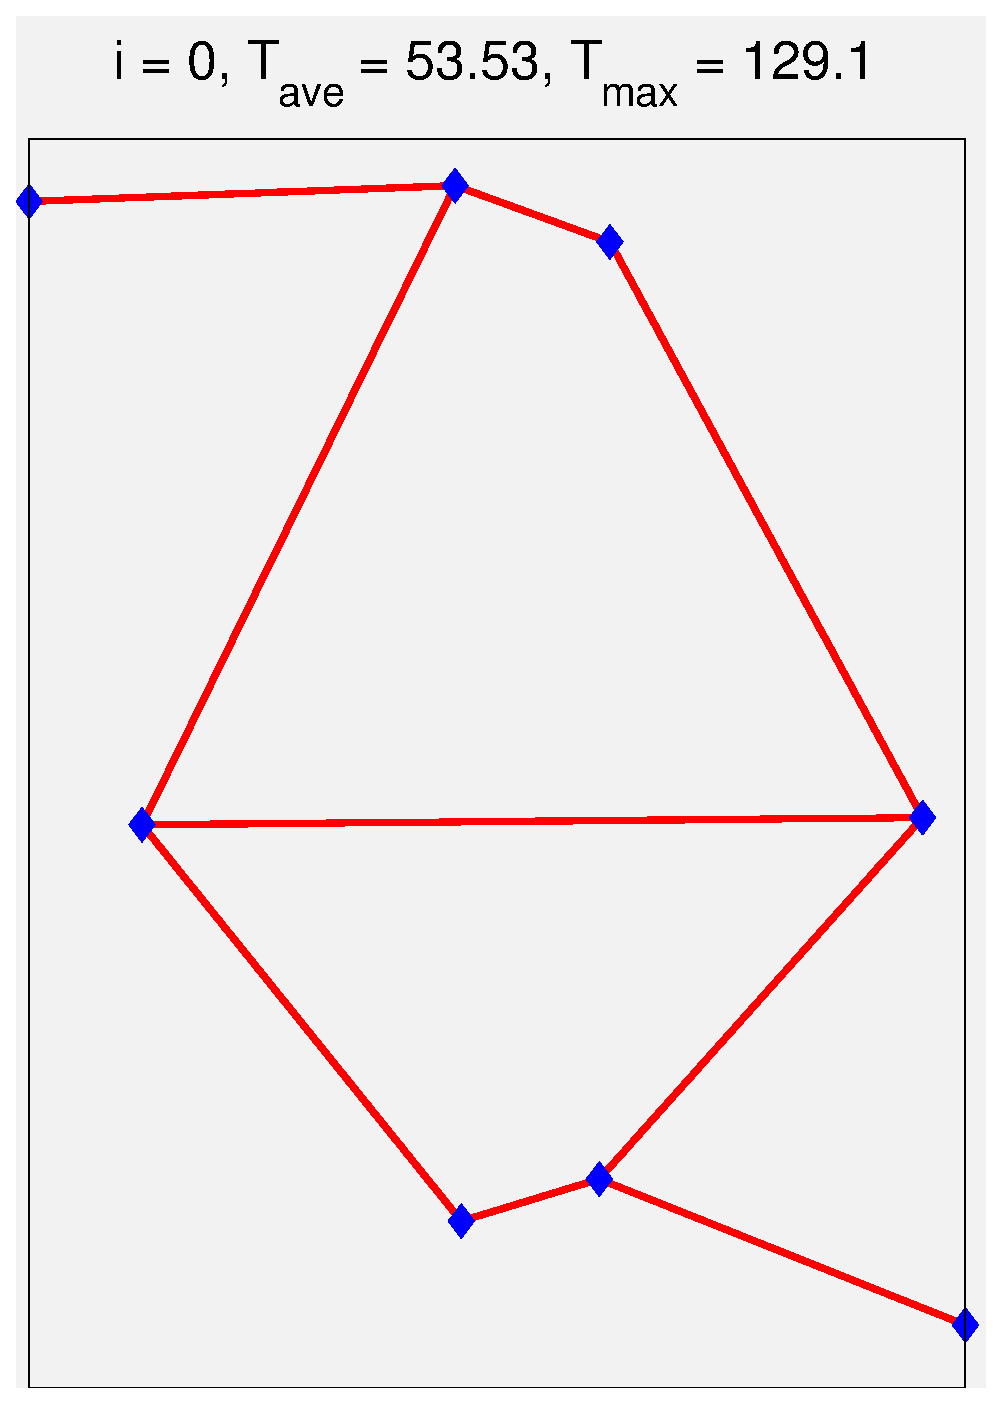
\includegraphics[width=\linewidth]{parallelTwo_Pmax30k_channel_0.eps}
\caption{}
\end{subfigure}
\begin{subfigure}{0.2\textwidth}
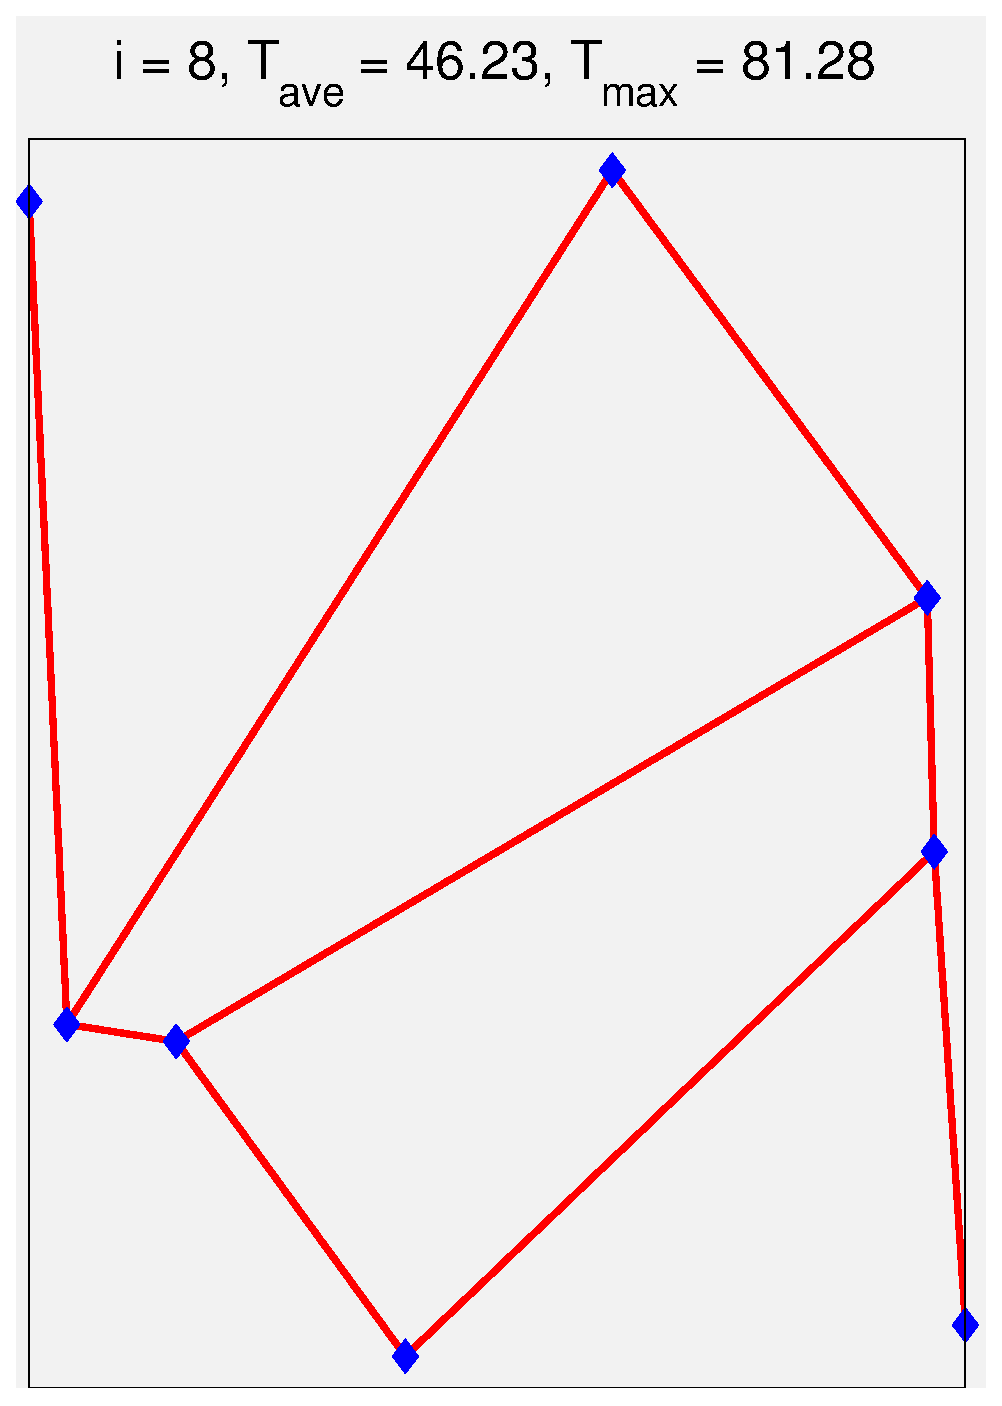
\includegraphics[width=\linewidth]{parallelTwo_Pmax30k_channel_8.eps}
\caption{}
\end{subfigure}
\begin{subfigure}{0.2\textwidth}
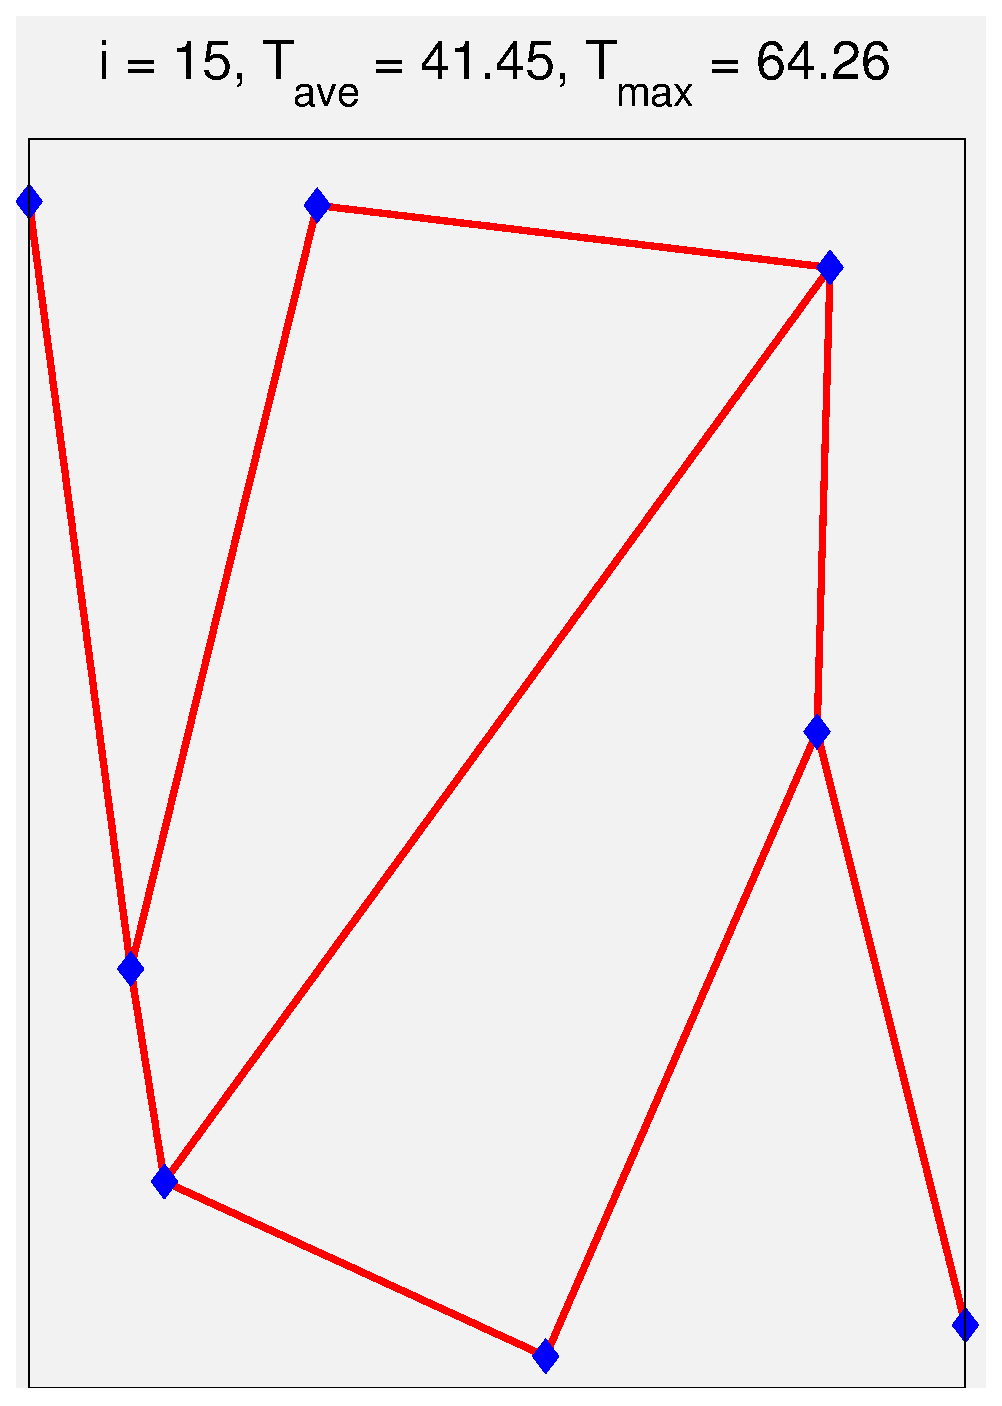
\includegraphics[width=\linewidth]{parallelTwo_Pmax30k_channel_15.eps}
\caption{}
\end{subfigure}
\begin{subfigure}{0.2\textwidth}
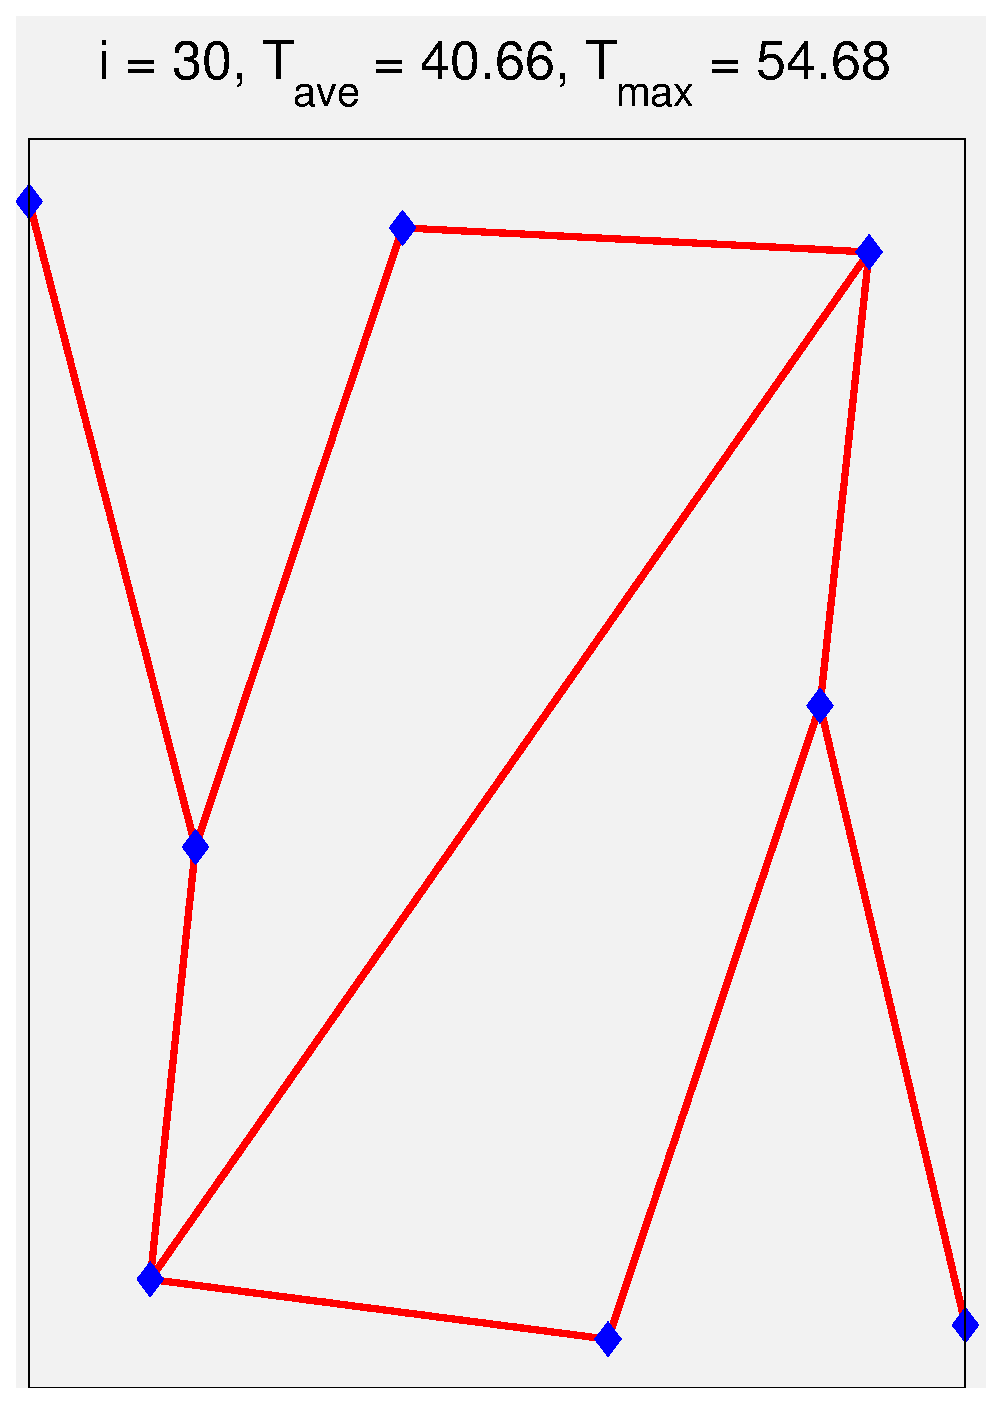
\includegraphics[width=\linewidth]{parallelTwo_Pmax30k_channel_30.eps}
\caption{}
\end{subfigure}

\centering
\begin{subfigure}{0.35\textwidth}
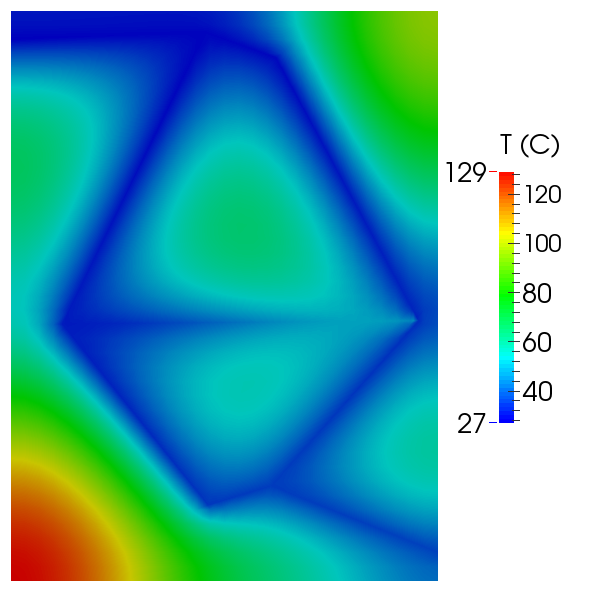
\includegraphics[width=\linewidth]{parallelTwo_T_0.png}
\caption{}
\end{subfigure}
\begin{subfigure}{0.35\textwidth}
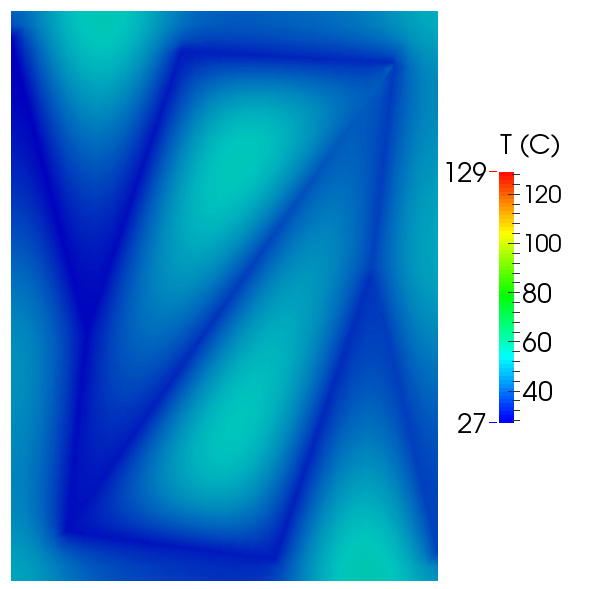
\includegraphics[width=\linewidth]{parallelTwo_T_30.png}
\caption{ }
\end{subfigure}

\centering
\begin{subfigure}{0.45\textwidth}
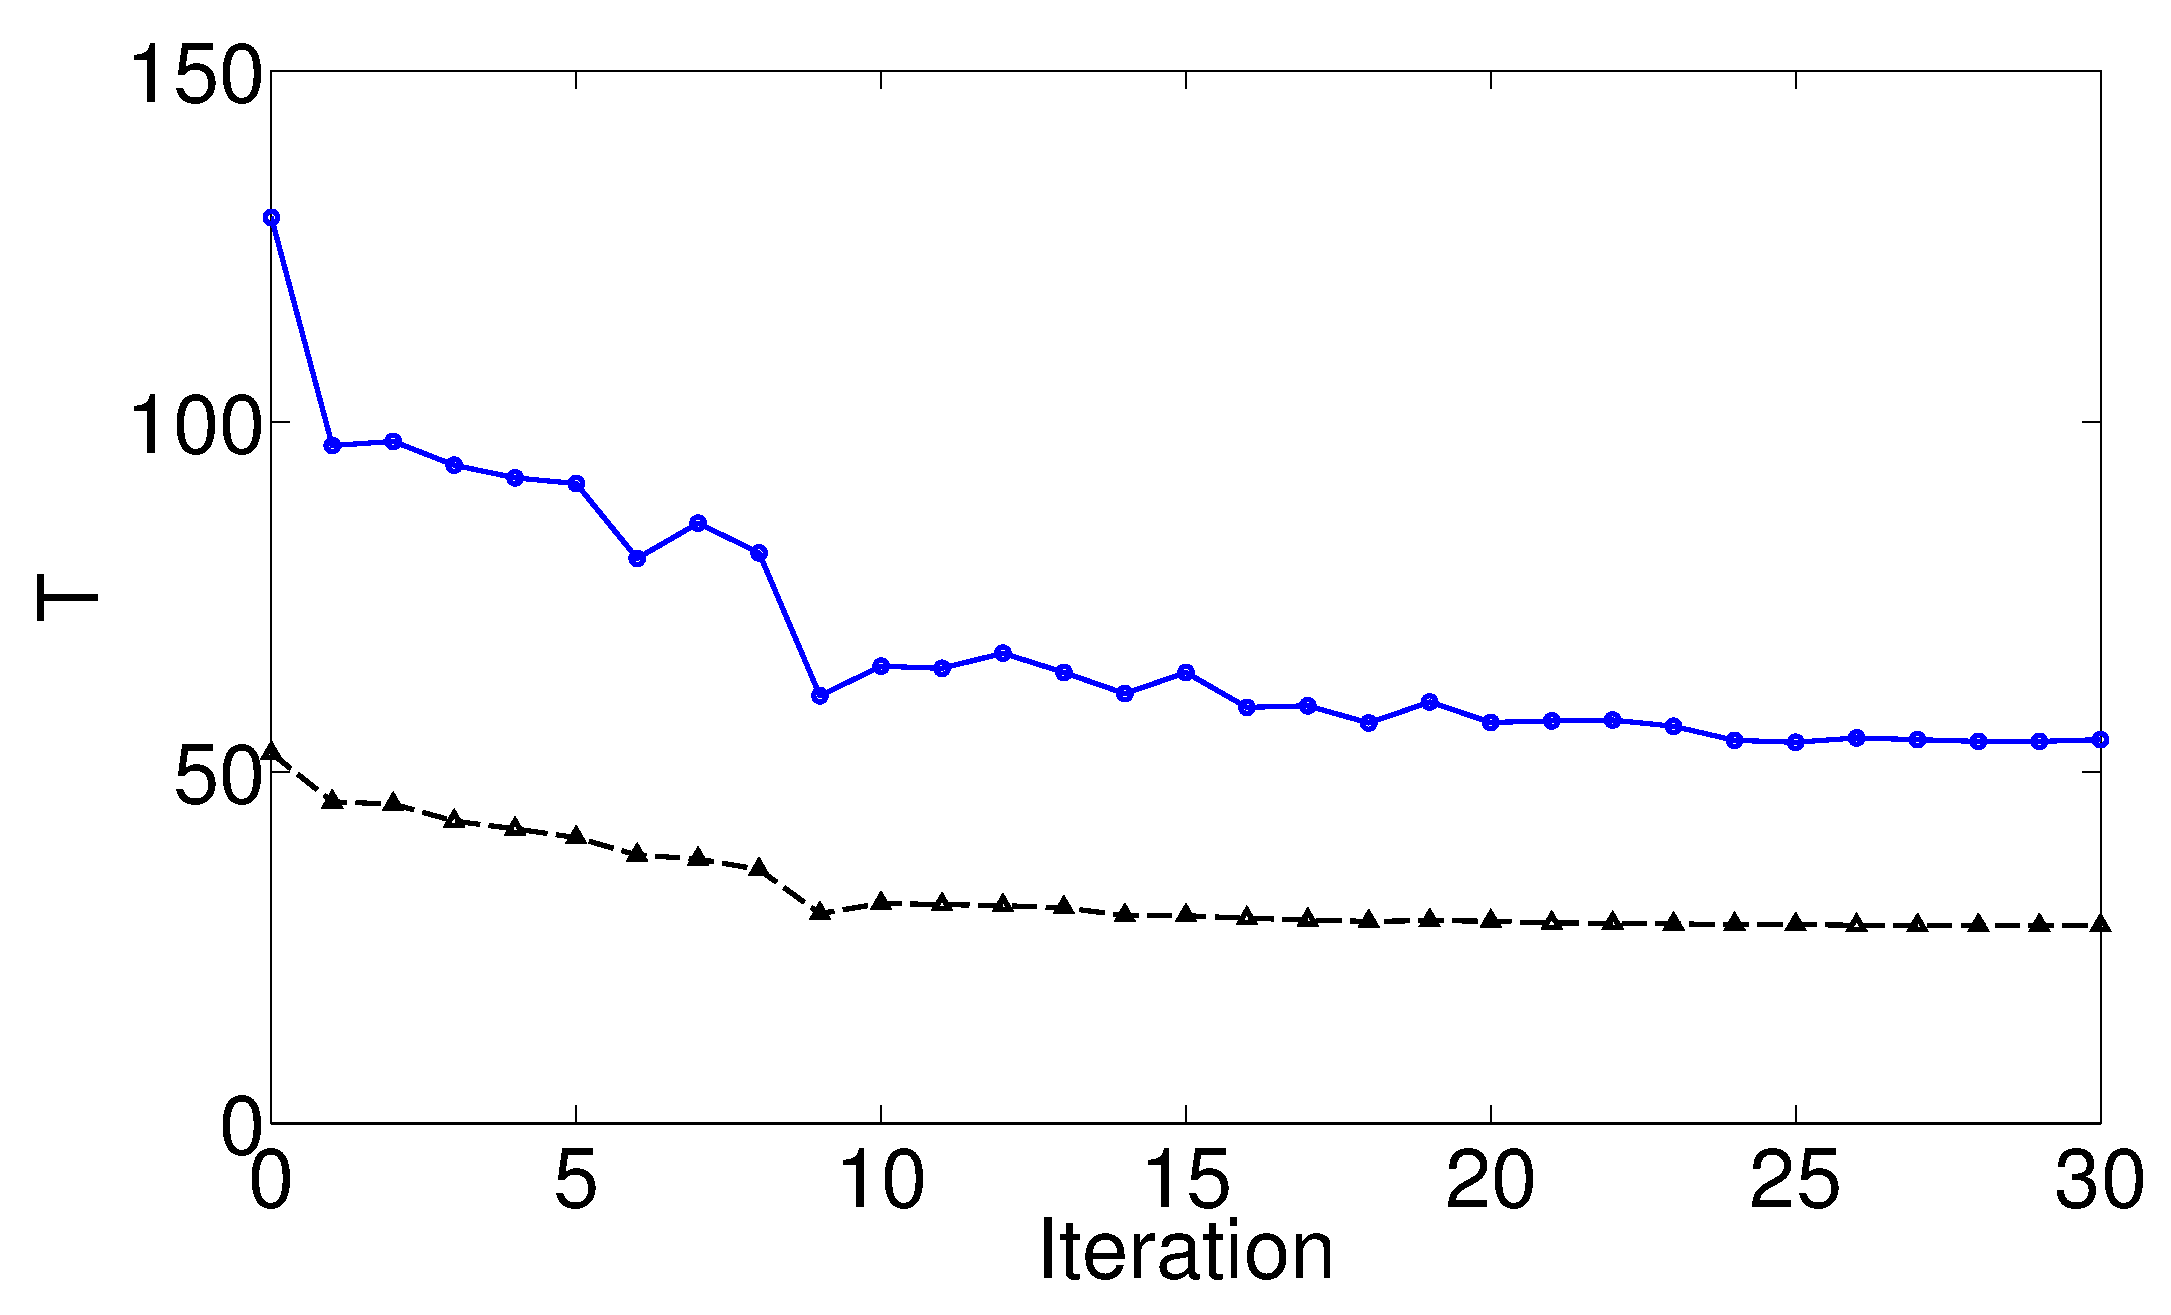
\includegraphics[width=\linewidth]{parallelTwo_Pmax30k_history.eps}
\caption{}
\end{subfigure}
\begin{subfigure}{0.4\textwidth}
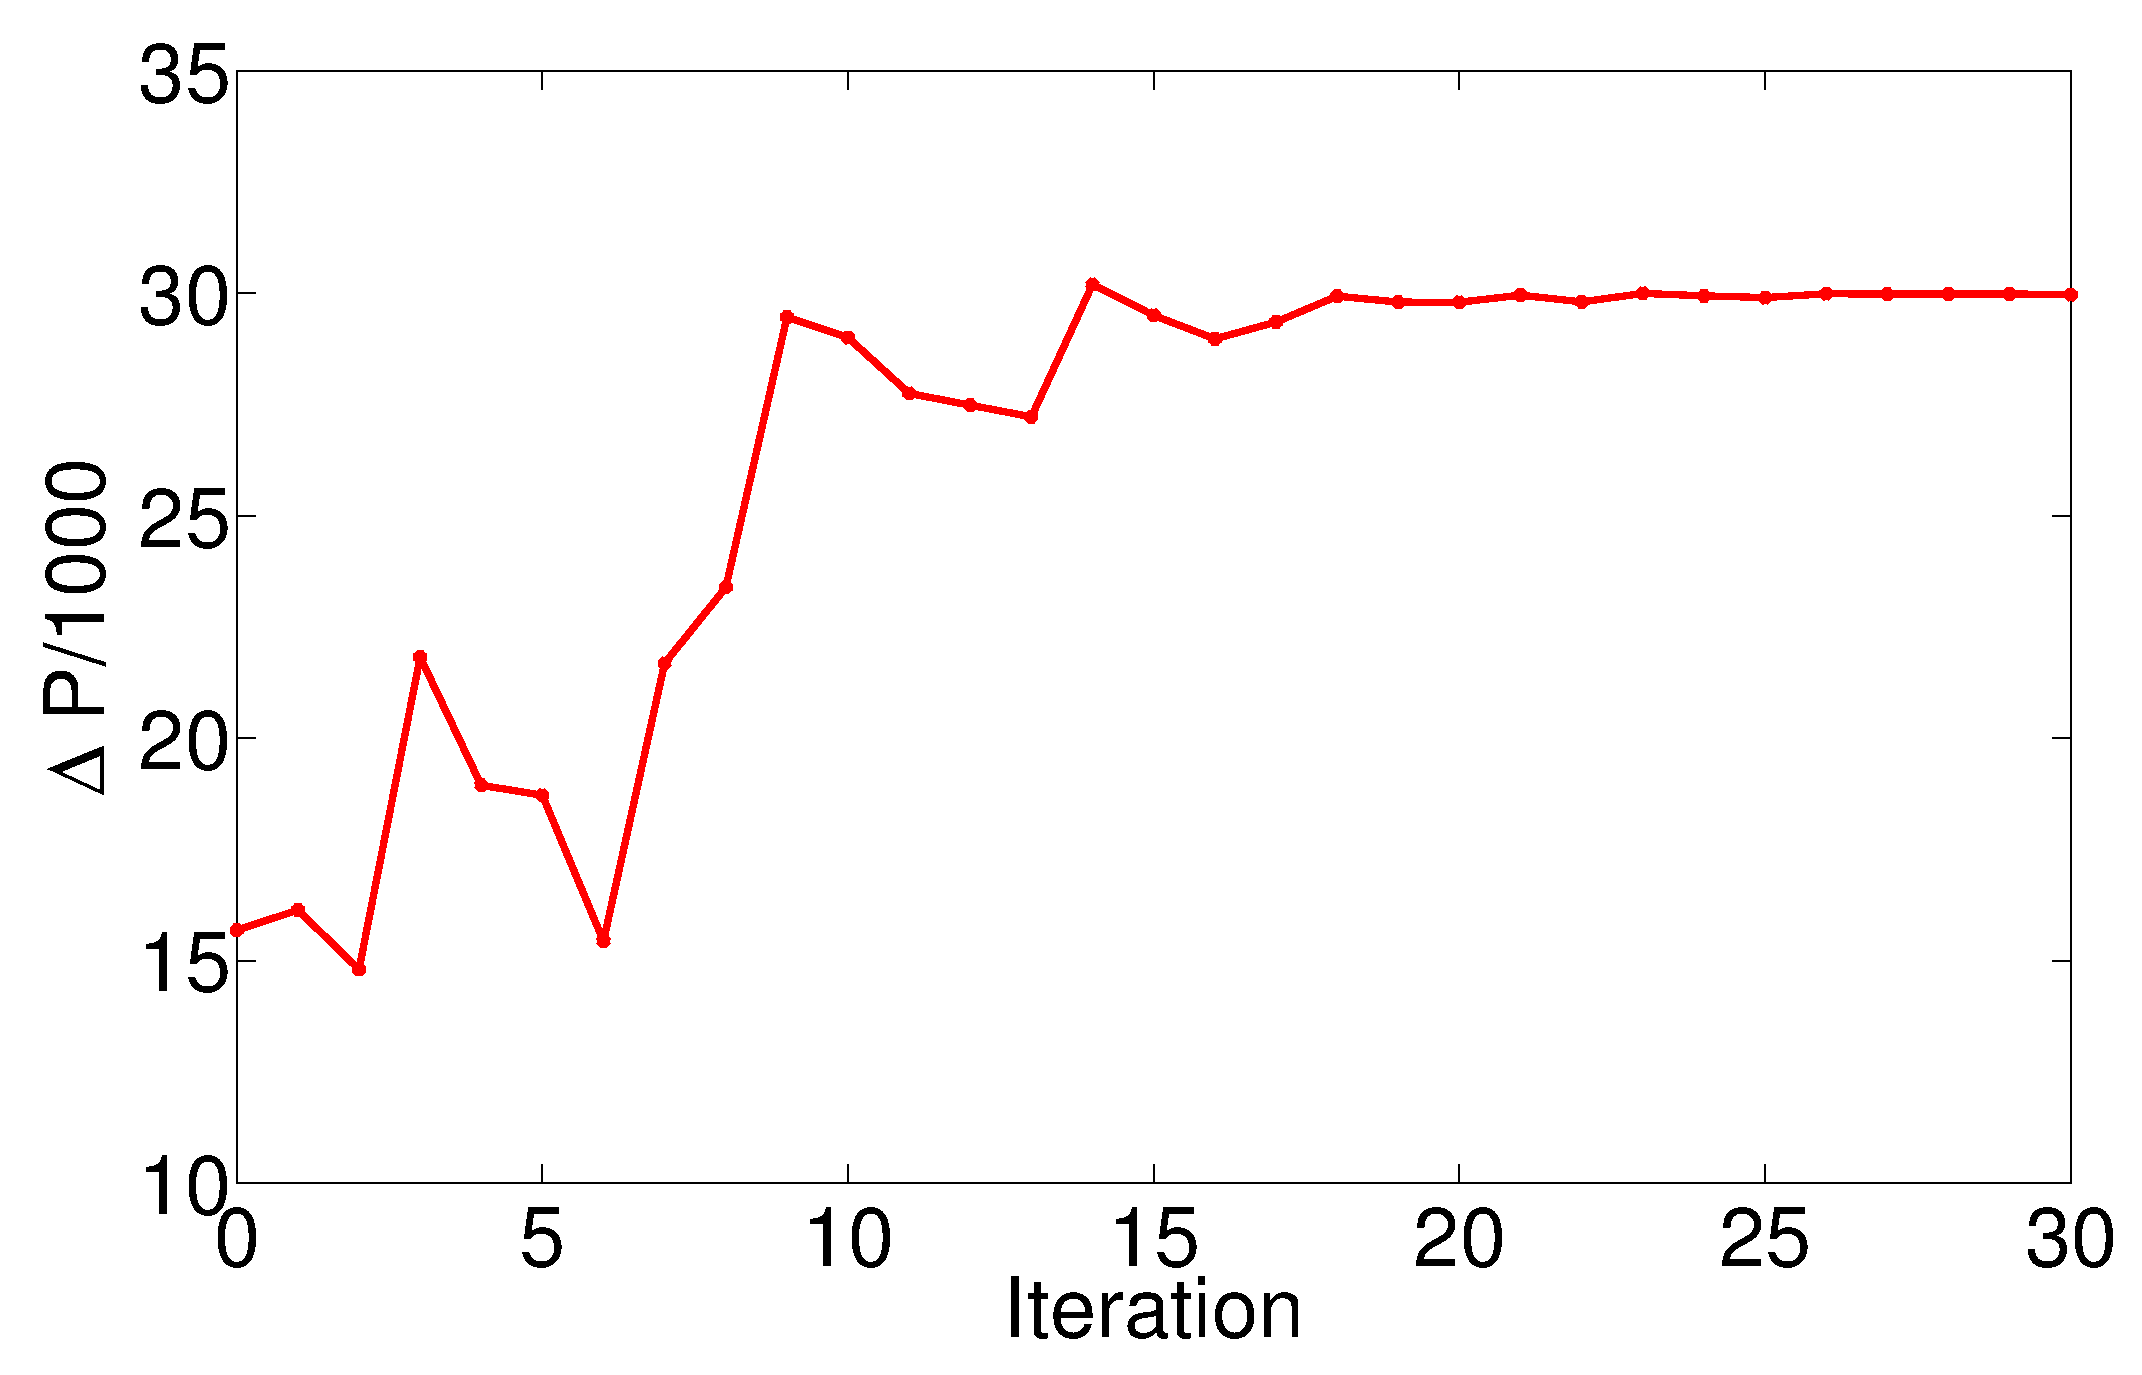
\includegraphics[width=\linewidth]{parallelTwo_Pmax30k_pressure_history.eps}
\caption{ }
\end{subfigure}

\caption{(a) - (d) Channel designs at iteration 0, 8, 15 and 30. (e), (f) The temperature distributions at iteration 0 and 30, obtained by plotting the generated vtk files in Paraview. (g) Histories of $T_{max}$ (blue circles with solid line) and 8-norm of temperature (black triangles with dashed line), and (g) pressure drop. }
\end{figure}

 
 \FloatBarrier
\subsection{Example 2: Generation of Pareto optimal front}
\label{subsec_Pareto_parallelTwo}
\begin{table}[!h]
\caption{Input arguments for Sec.\ \ref{subsec_Pareto_parallelTwo}.  Blank arguments are not applicable. SI units are used for all quantities except temperature, which is in \degree C.}
\label{tab_generate_pareto_front_inputs1}
\centering
\begin{tabular}{|c|c|}
\hline
Argument \# & Value \\
\hline
1 & `parallelTwoNEoptimal.channel'\\
\hline
2 & `parallelTwo\texttt{\_}NE.polygon' \\
\hline
3 & `parallel2Pareto' \\
\hline
4 &  `parallelTwoPareto' \\
\hline
5 & [30,40] \\
\hline
6 & [0,0.15,0,0.2] \\
\hline
7 & `T,P' \\
\hline
8 & 8 \\
\hline
9 & [25.49,246.5; 46994,261]\\
\hline
10 & 60 \\
\hline
11 & [ ] \\
\hline
12 & \\
\hline
13 & \\
\hline
14 & \\
\hline
15 & \\
\hline
16 & \\
\hline
17 & false \\
\hline 
18 & 2.7 \\
\hline 
19 & 0.003 \\
\hline
20 & 0 \\
\hline 
21 & 0 \\
\hline
22 & 500  \\
\hline
\end{tabular}
\end{table}

\begin{figure}[!h]
\centering
\begin{subfigure}{0.2\textwidth}
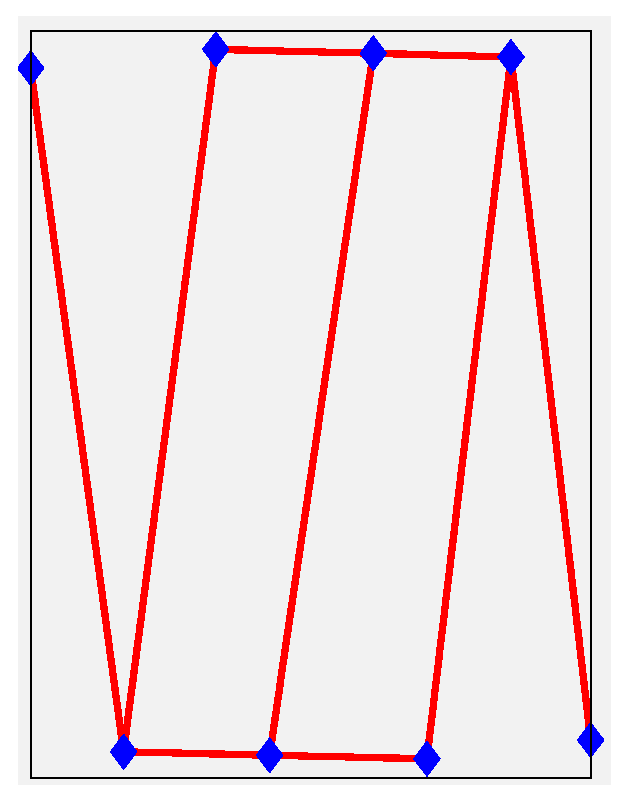
\includegraphics[width=\linewidth]{parallelTwoPareto_sim0_minT8.eps}
\caption{}
\end{subfigure}
\begin{subfigure}{0.2\textwidth}
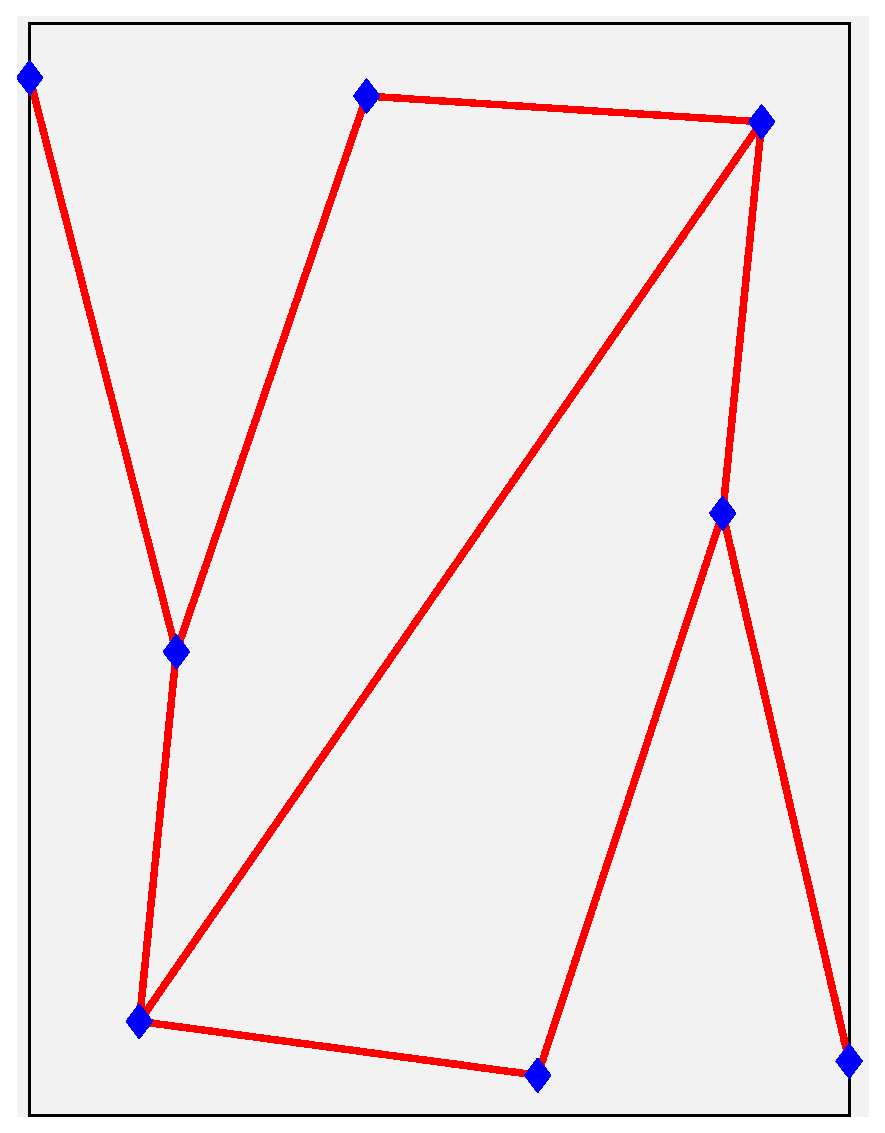
\includegraphics[width=\linewidth]{parallelTwoPareto_sim12.eps}
\caption{}
\end{subfigure}
\begin{subfigure}{0.2\textwidth}
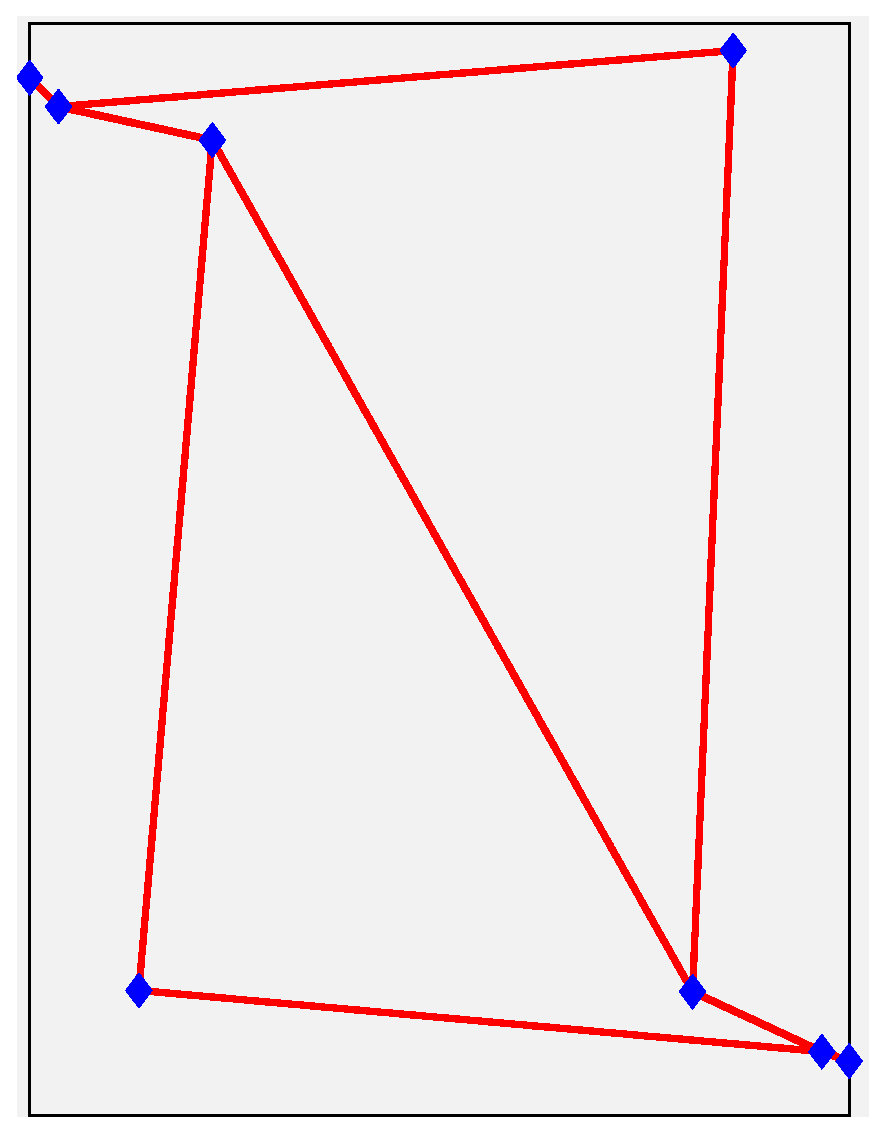
\includegraphics[width=\linewidth]{parallelTwoPareto_sim25.eps}
\caption{}
\end{subfigure}
\begin{subfigure}{0.2\textwidth}
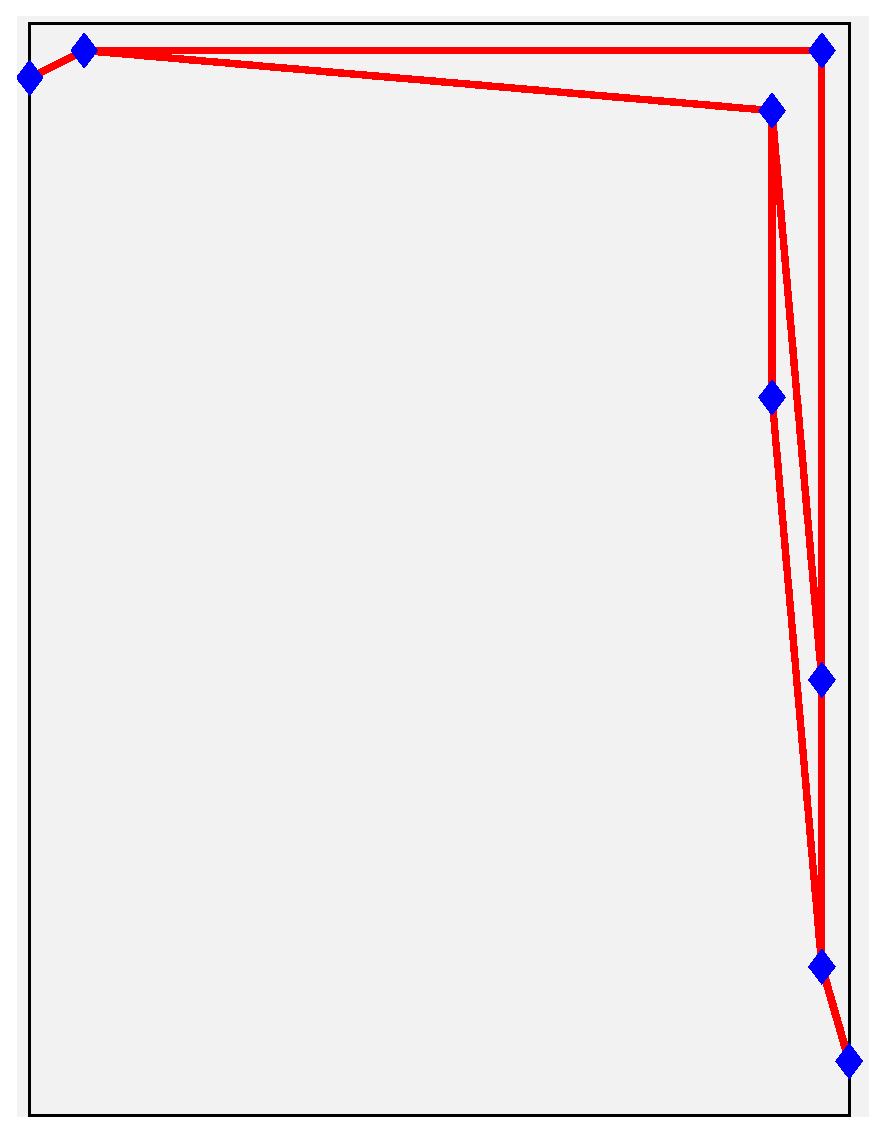
\includegraphics[width=\linewidth]{parallelTwoPareto_sim60_minP_Aminp018.eps}
\caption{}
\end{subfigure}

\begin{subfigure}{0.8\textwidth}
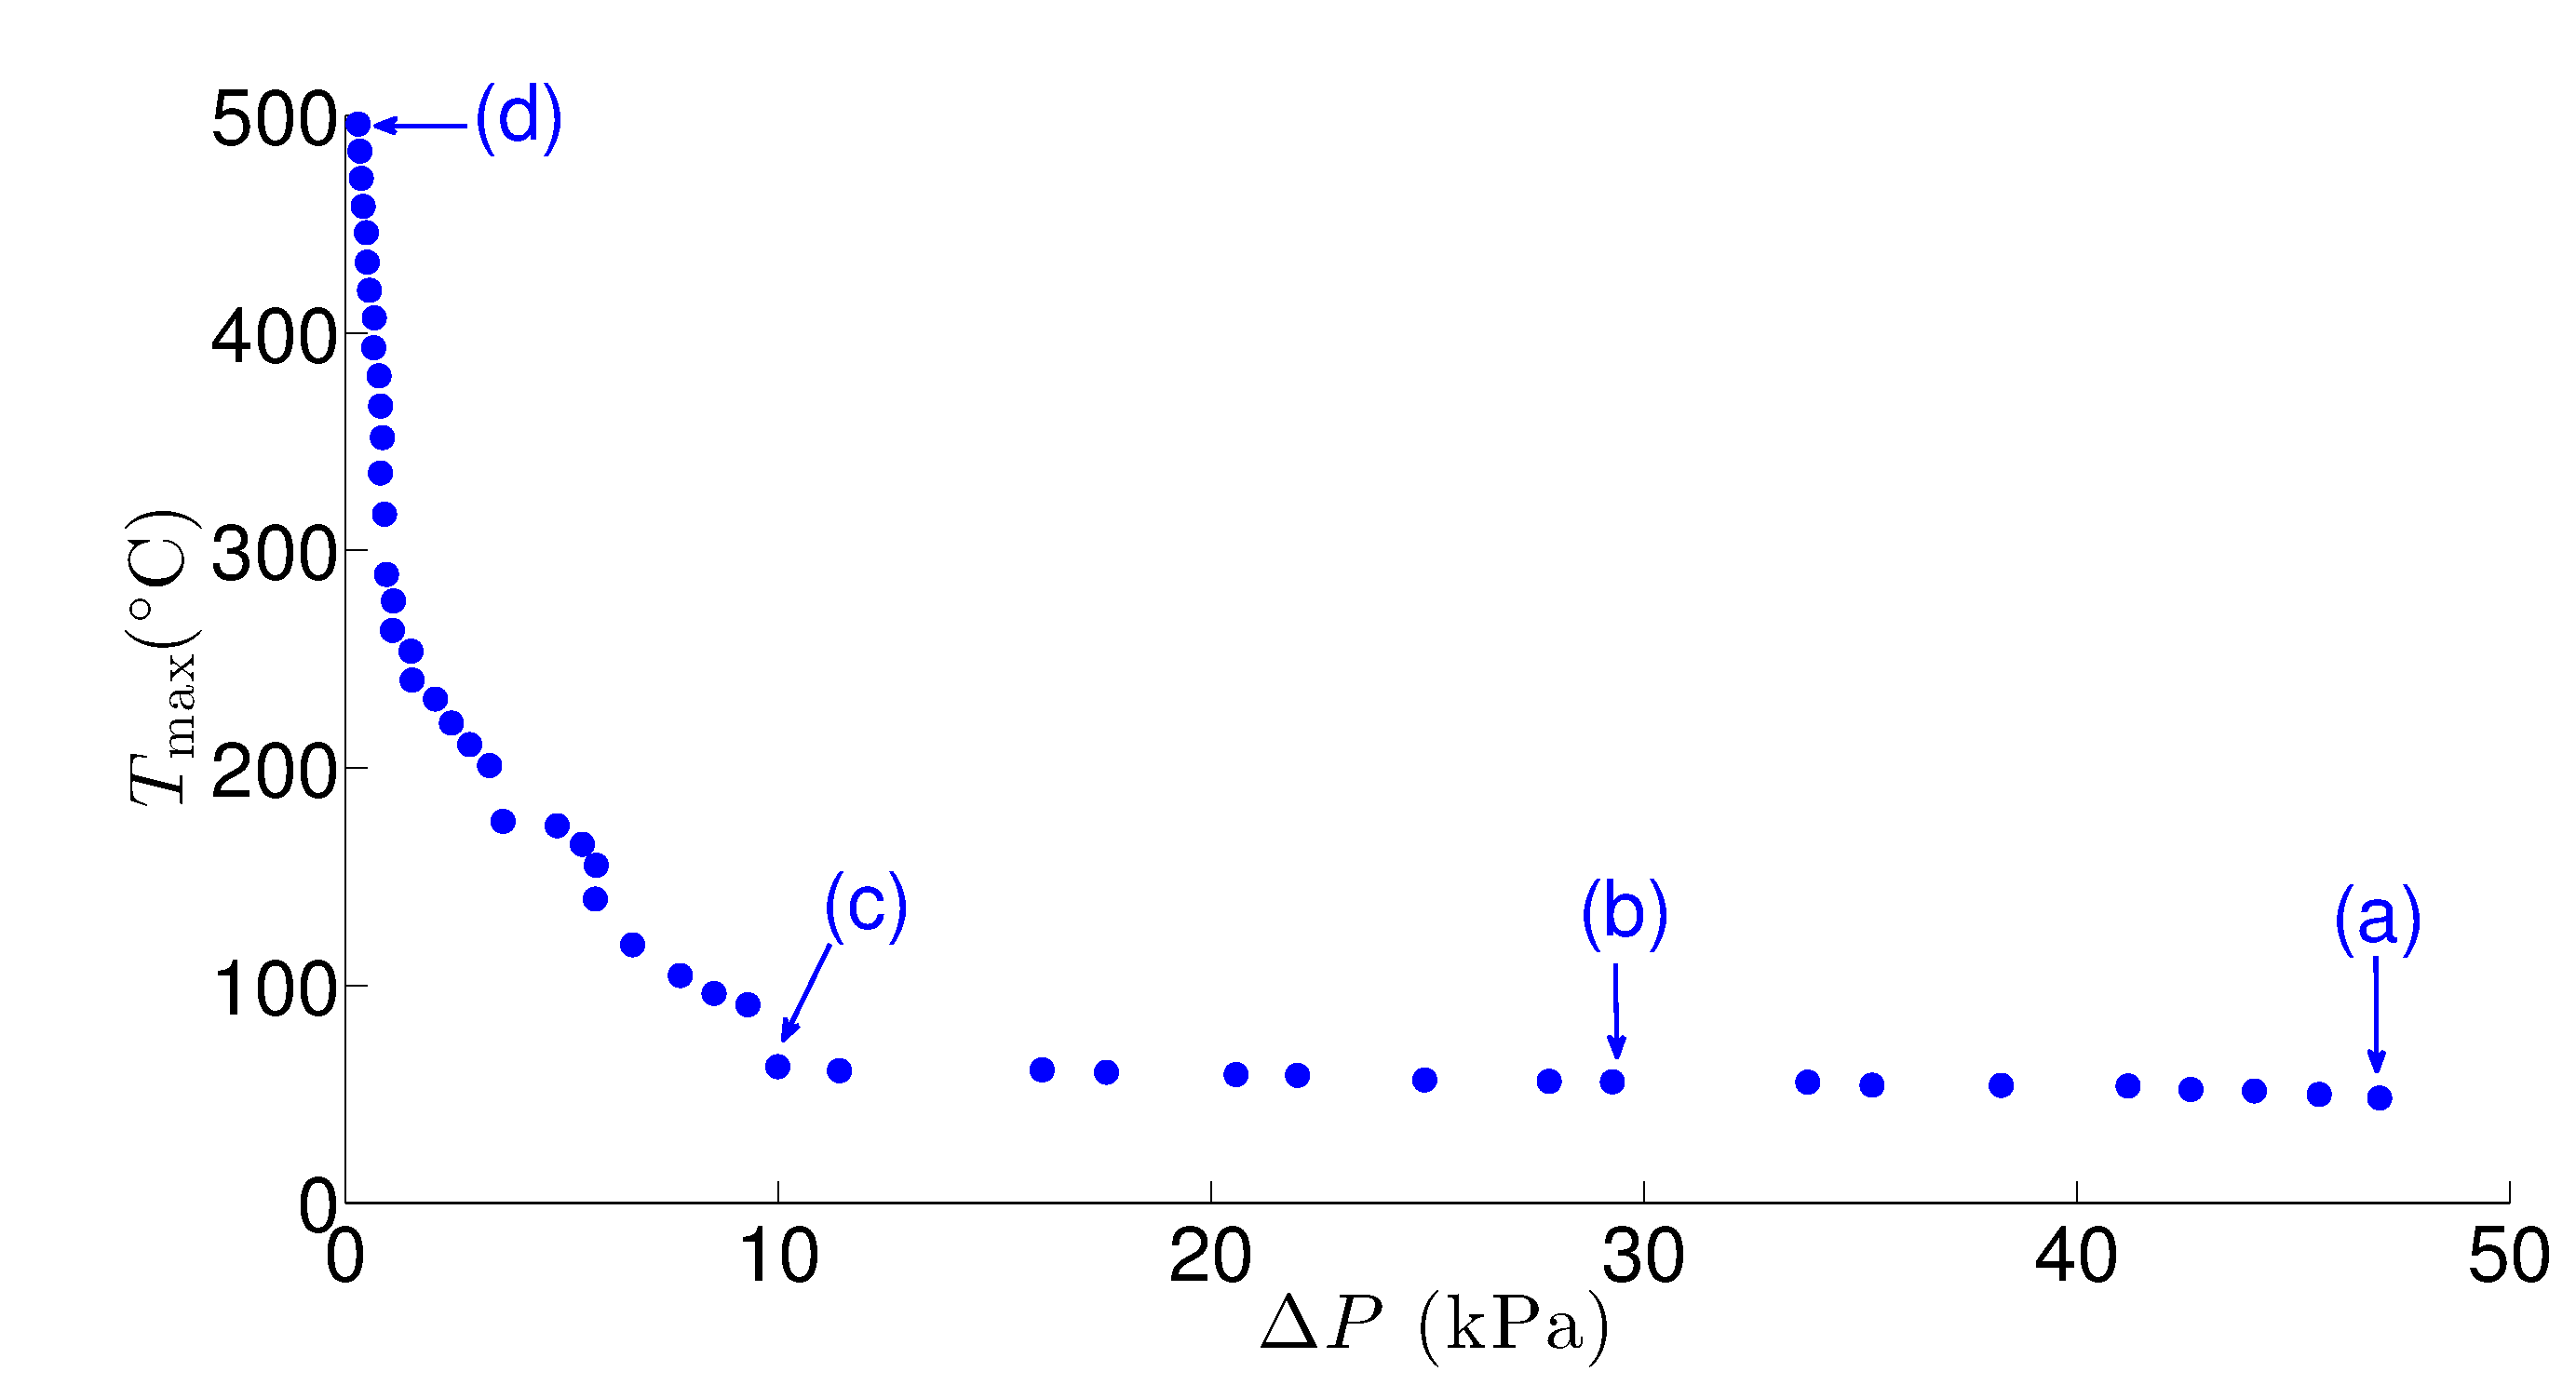
\includegraphics[width=\linewidth]{parallelTwoPareto_60pts.eps}
\caption{}
\end{subfigure}
\caption{(a) Optimal design resulting from minimizing the 8-norm alone. (b), (c) Optimal designs along the Pareto front in (e).(d) Optimal design resulting from minimizing the pressure drop subject to a minimum area fraction of 0.018. (e) $T_{max}$-$\Delta P$ Pareto front obtained by postprocessing the 8-norm-$\Delta P$ Pareto points and filtering the resulting points using a Pareto filter. }
\end{figure}

\FloatBarrier
\subsection{Example 3: Optimization of `worst-case scenario'}
\label{subsec_worst_cast_parallel2x2}

\begin{table}[!h]
\caption{Input arguments for \texttt{optimize\_blocked\_channels.m}.}
\label{tab_optimize_blocked_channels_inputs1}
\centering
\begin{tabular}{|c|c|}
\hline
Argument \# & Description\\
\hline
1 & `parallel2x2ref.channel' \\
\hline
2 & `parallel2x2NE.polygon'\\
\hline
3 & `parallel2x2\texttt{\_}1xp1\texttt{\_}a.rand'\\  
\hline
4 & `parallel2x2nBlk1.blk' \\
\hline
5 & -22 \\
\hline
6 & `parallel2x2'\\
\hline
7 &`insulated\texttt{\_}composite'  \\
\hline
8 & [40,40]  \\
\hline
9 & [0,0.05,0,0.05] \\
\hline
10 & 'P\texttt{\_}NORM'  \\
\hline
11 & 8  \\
\hline
12 & [ ] \\
\hline
13 & \\
\hline
14 & \\
\hline
15 & \\
\hline
16 & \\
\hline
17 & \\
\hline
18 & 1 \\
\hline
19 & false \\
\hline
20 & false \\
\hline 
21 & 2.7  \\
\hline 
22 & 0.003 \\
\hline
23 & 0 \\
\hline 
24 & 0 \\
\hline
25 & 500 \\
\hline
\end{tabular}
\end{table}

\begin{figure}[!h]
\centering
\begin{subfigure}{0.2\textwidth}
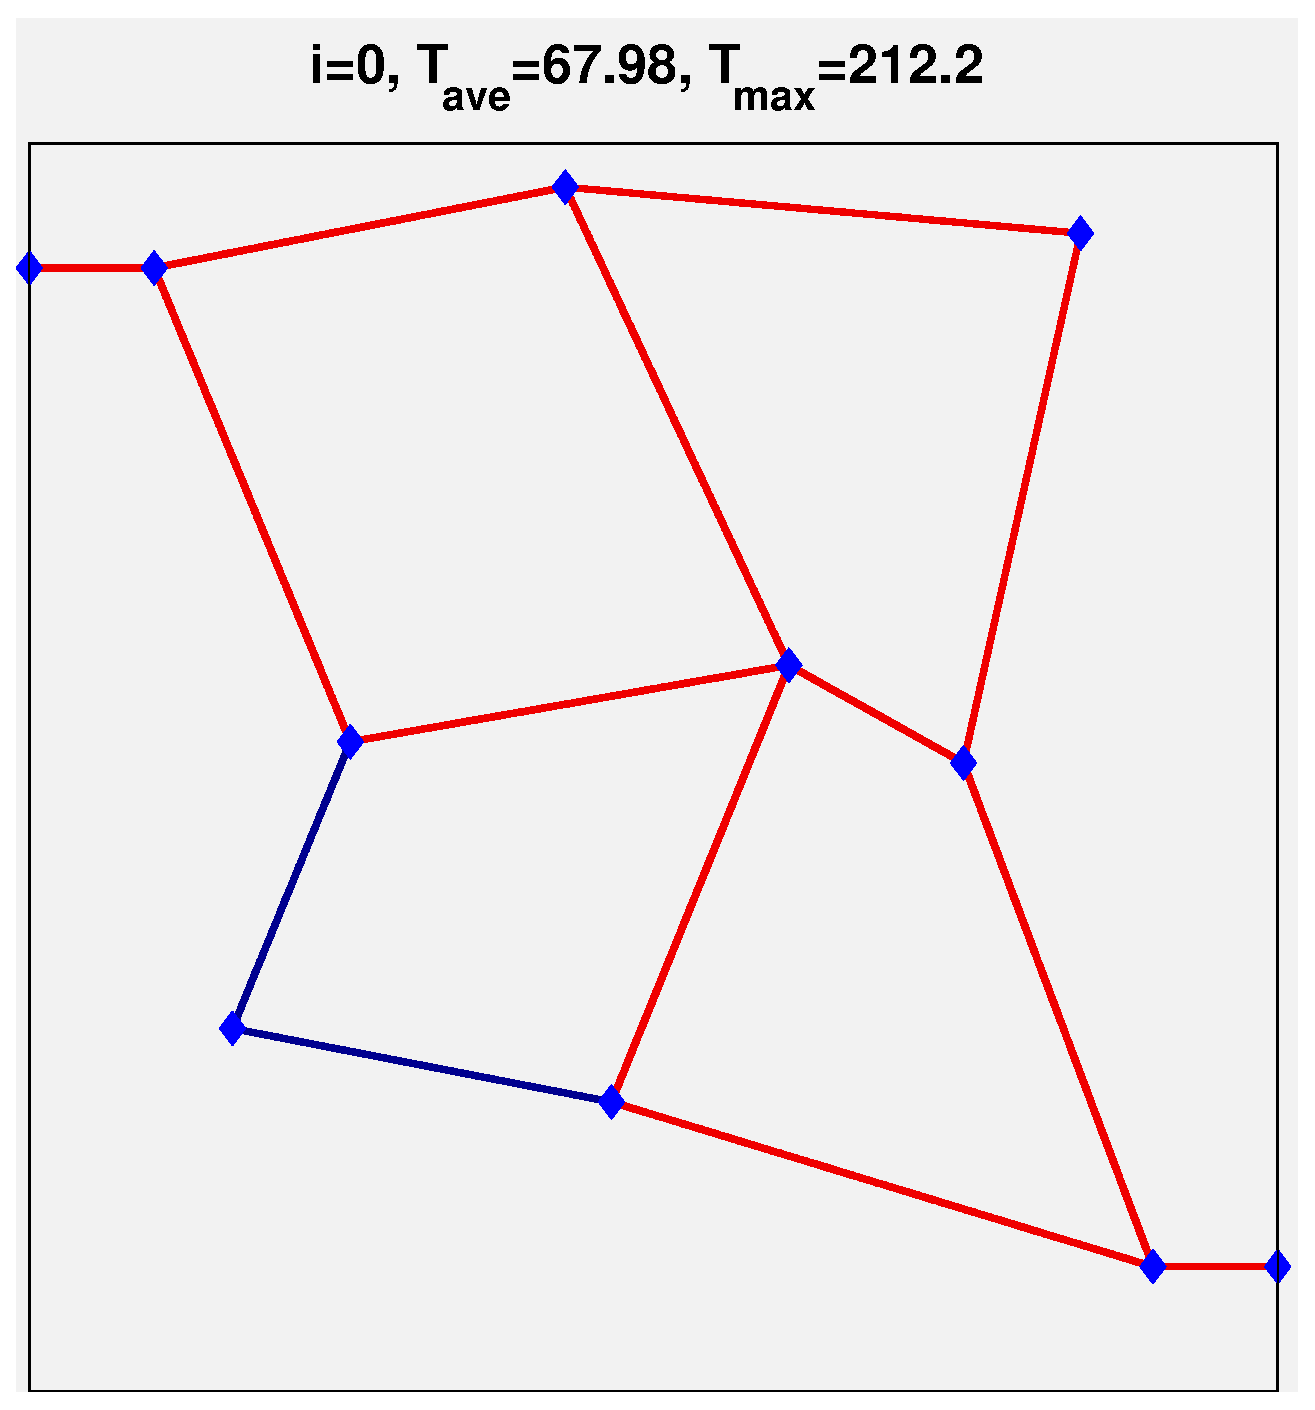
\includegraphics[width=\linewidth]{parallel2x2_channel_0.eps}
\caption{}
\end{subfigure}
\begin{subfigure}{0.2\textwidth}
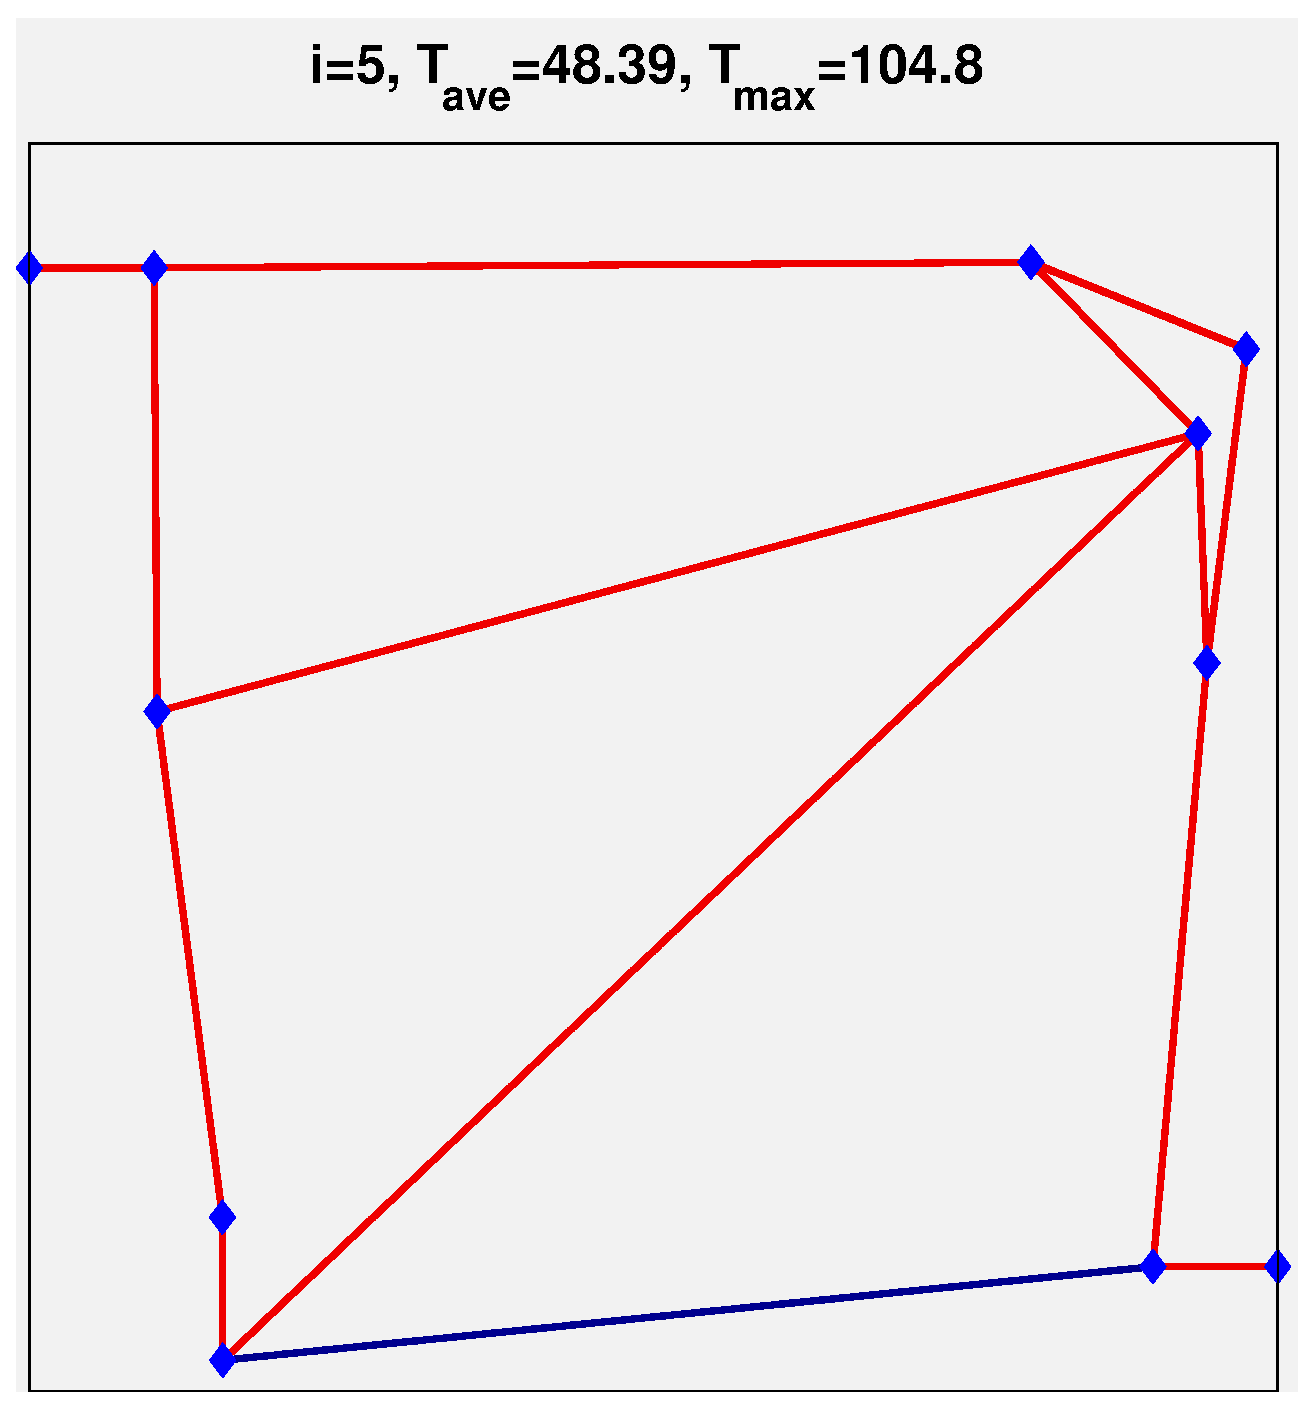
\includegraphics[width=\linewidth]{parallel2x2_channel_5.eps}
\caption{}
\end{subfigure}
\begin{subfigure}{0.2\textwidth}
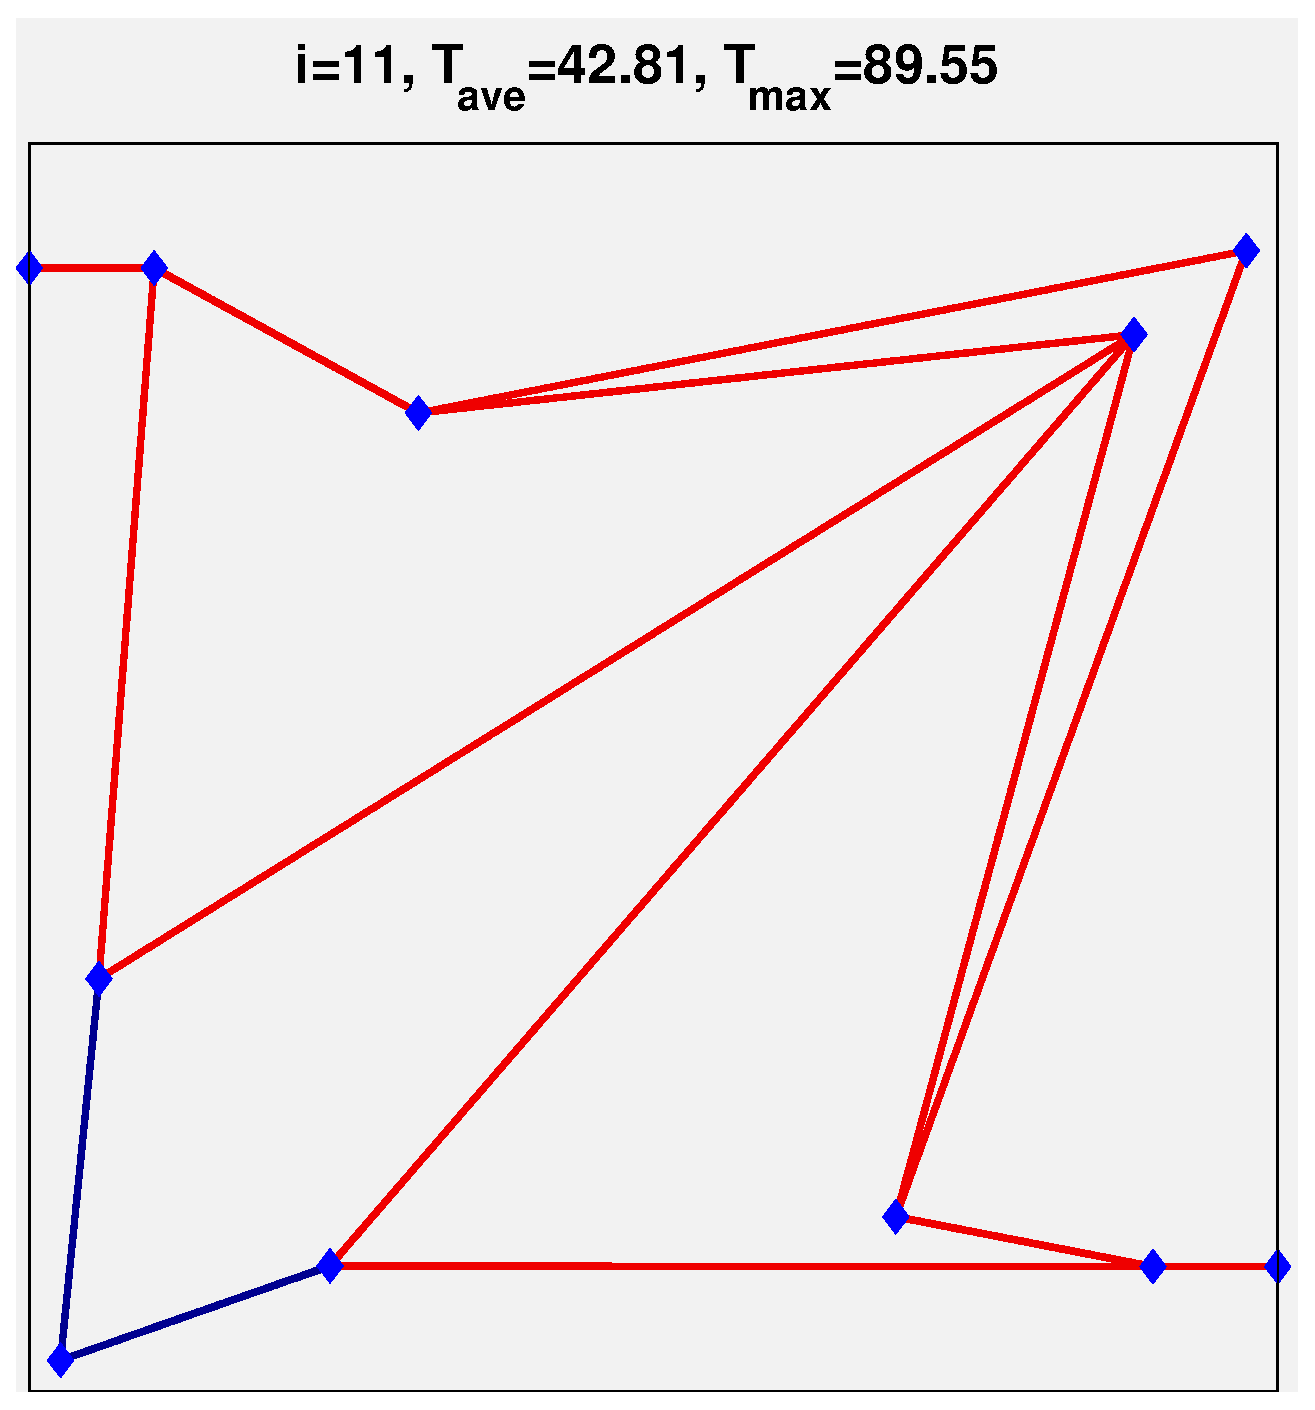
\includegraphics[width=\linewidth]{parallel2x2_channel_11.eps}
\caption{}
\end{subfigure}
\begin{subfigure}{0.2\textwidth}
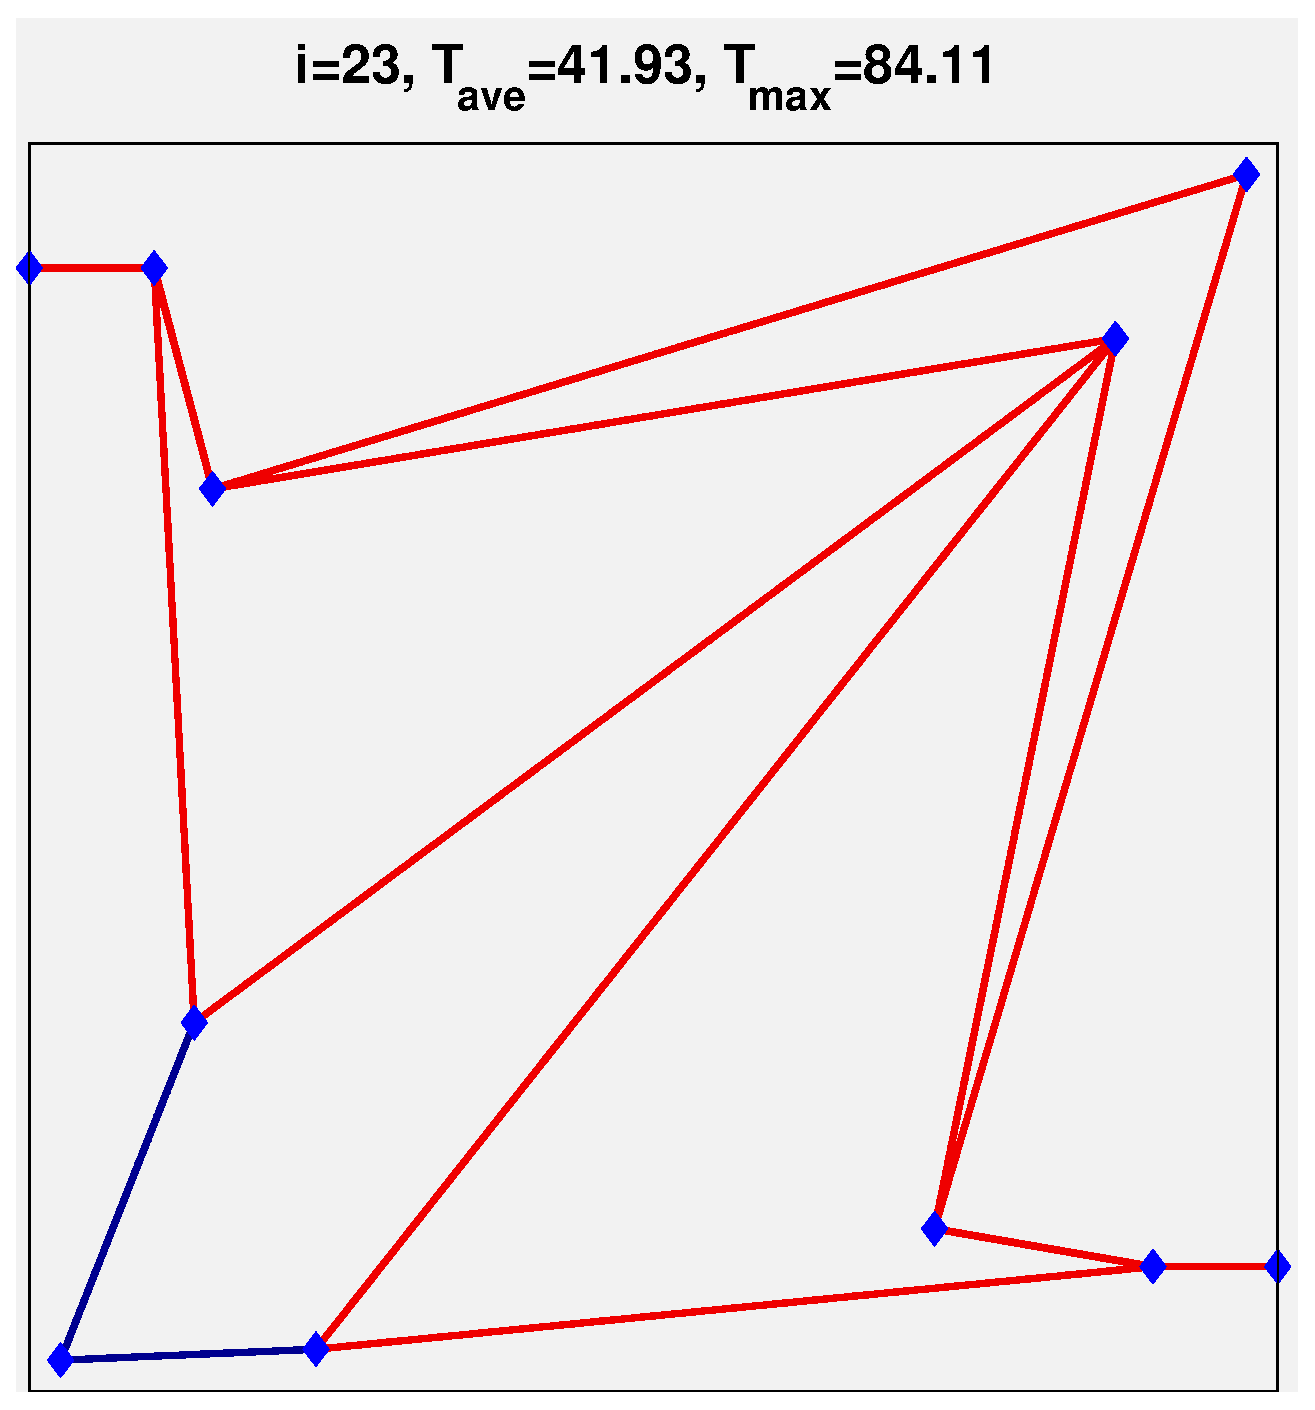
\includegraphics[width=\linewidth]{parallel2x2_channel_23.eps}
\caption{}
\end{subfigure}

\begin{subfigure}{0.4\textwidth}
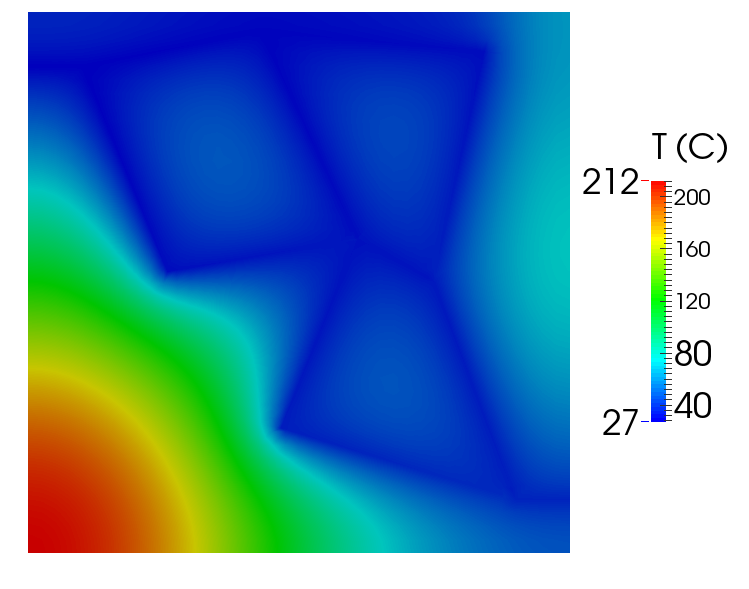
\includegraphics[width=\linewidth]{parallel2x2_T_0.png}
\caption{}
\end{subfigure}
\begin{subfigure}{0.4\textwidth}
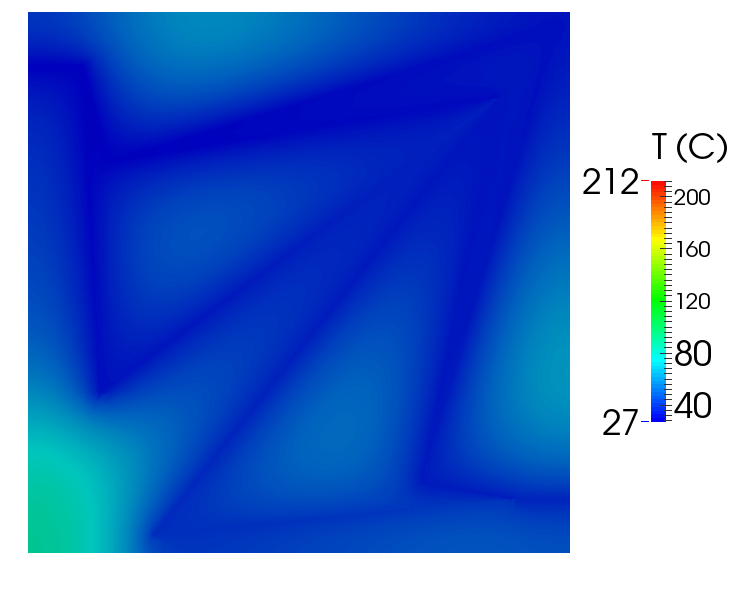
\includegraphics[width=\linewidth]{parallel2x2_T_23.png}
\caption{}
\end{subfigure}

\begin{subfigure}{0.41\textwidth}
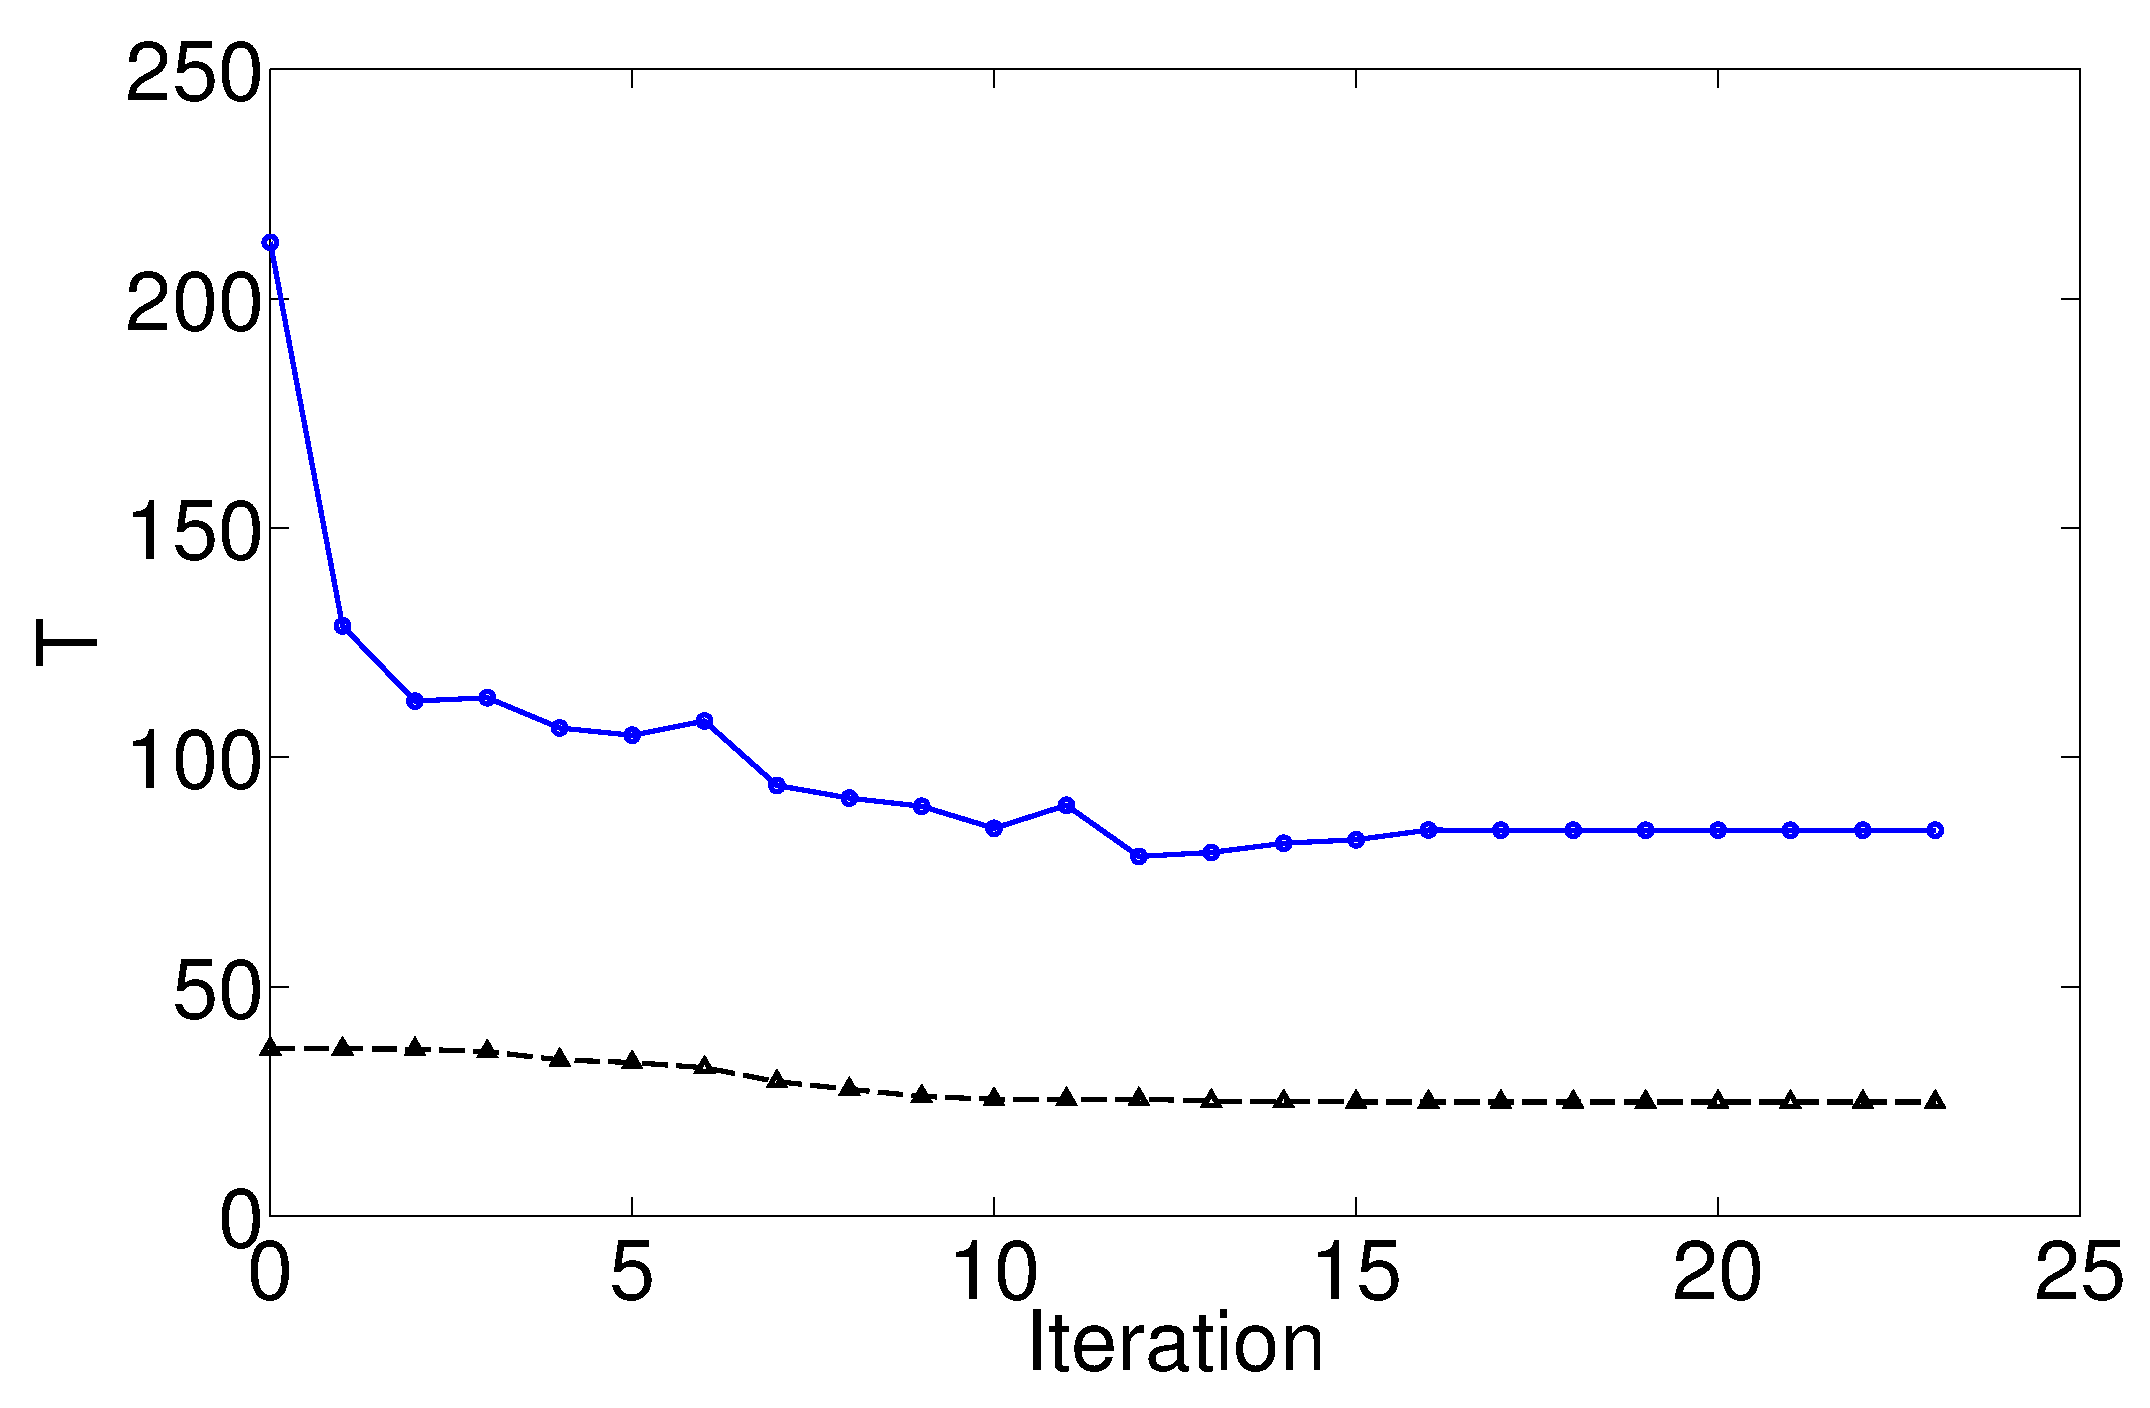
\includegraphics[width=\linewidth]{parallel2x2_history.eps}
\caption{}
\end{subfigure}
\begin{subfigure}{0.42\textwidth}
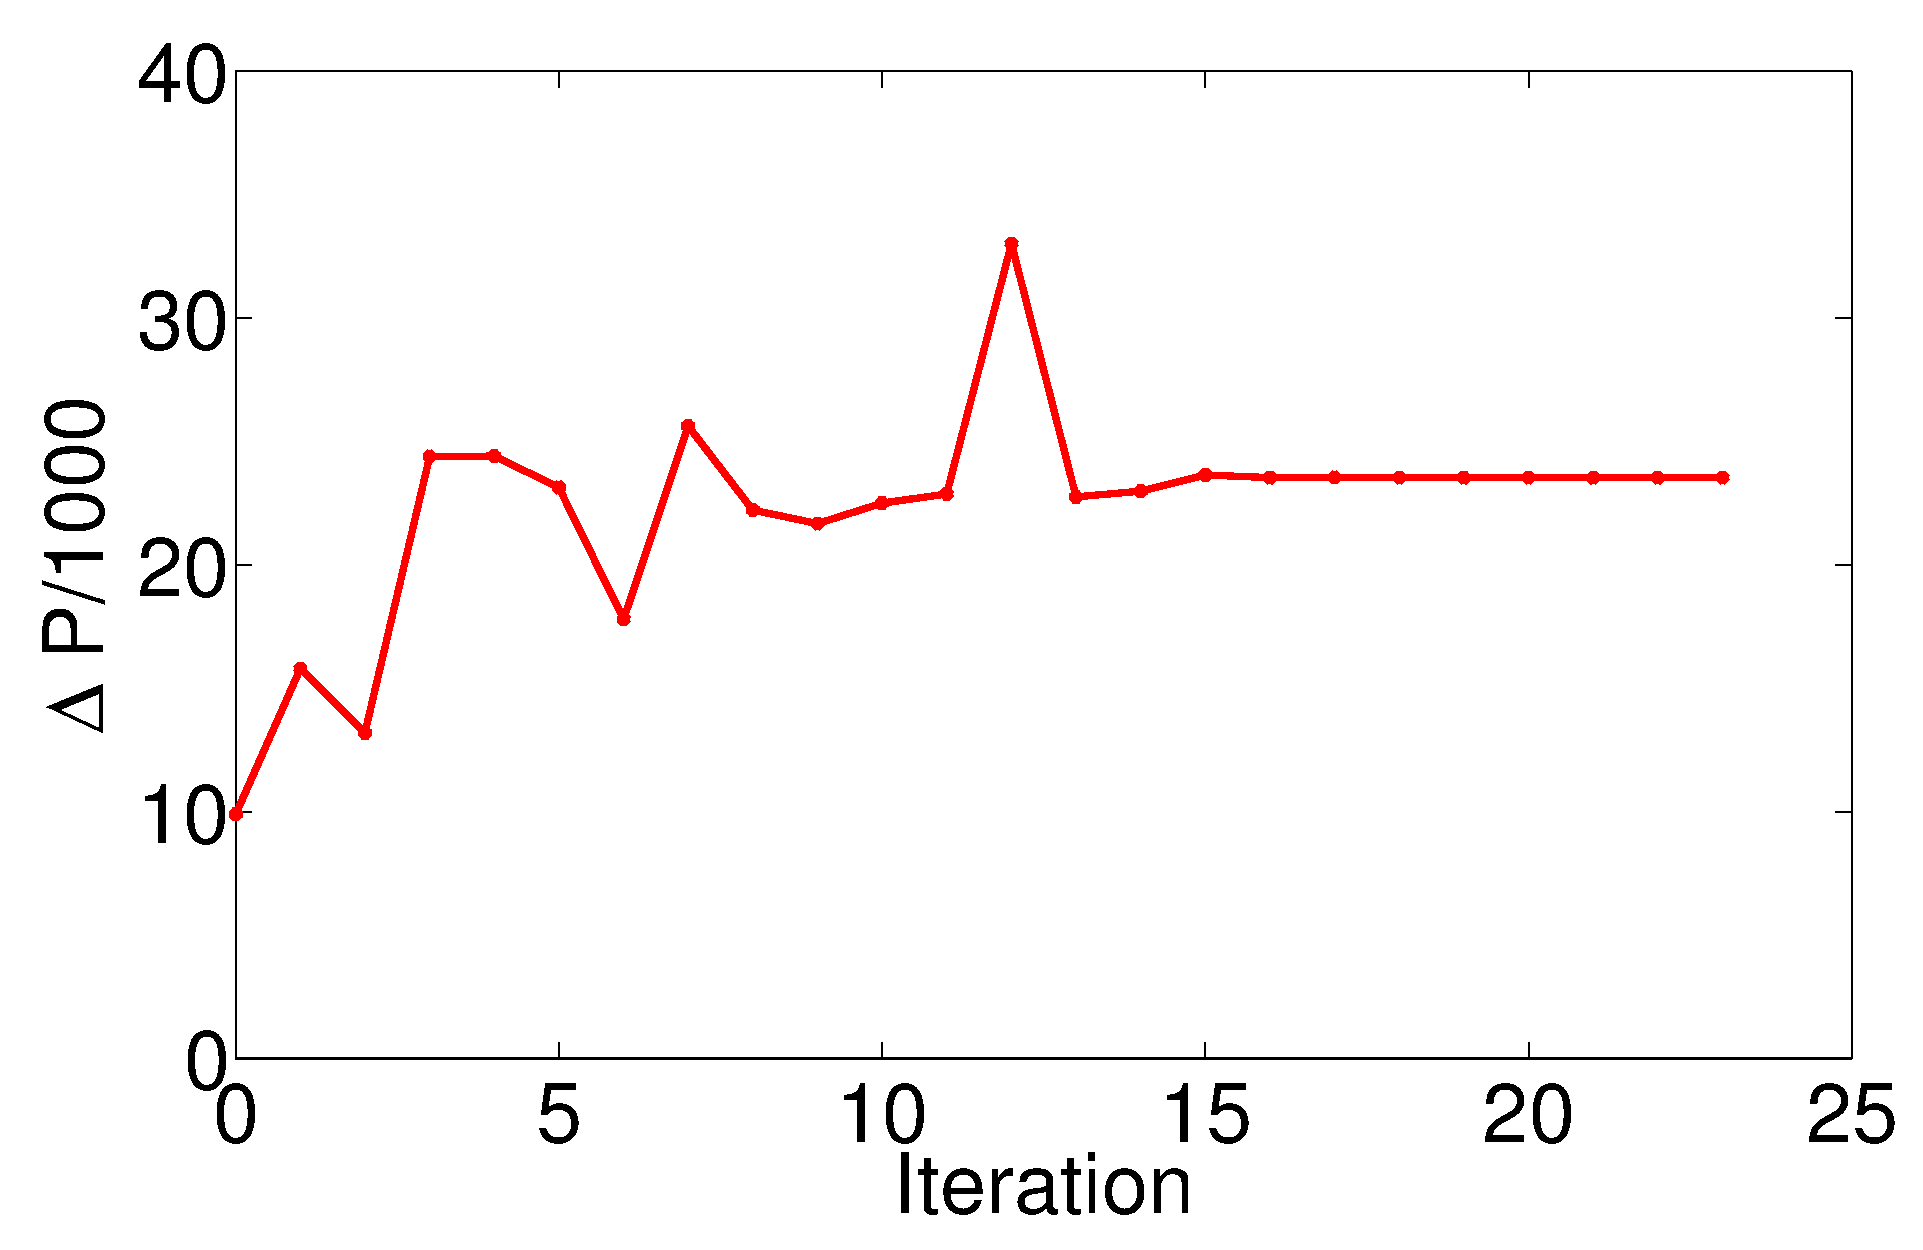
\includegraphics[width=\linewidth]{parallel2x2_pressure_history.eps}
\caption{}
\end{subfigure}
\caption{(a) - (d) Channel designs at iteration 0, 5, 11 and 23. (e), (f) The temperature distributions at iteration 0 and 30, obtained by plotting the generated vtk files in Paraview. (g) Histories of $T_{max}$ (blue circles with solid line) and 8-norm of temperature (black triangles with dashed line), and (h) pressure drop. }
\end{figure}


\FloatBarrier

\section{References}
\bibliographystyle{plainnat}
\bibliography{references}    
\end{document}
